%Preamble
\documentclass[12pt,a4paper]{article}        %Define text type and basic formatting
\usepackage[margin=1.25in]{geometry}
%\usepackage[document]{ragged2e}   %Text alignment https://www.overleaf.com/learn/latex/Text_alignment
\usepackage{microtype}  %Refined word breaks

\usepackage{tcolorbox} %Bordered boxes
\usepackage{float}

\usepackage[utf8]{inputenc}     %Usage of UTF-8 for umlauts
\usepackage[ngerman]{babel}     %Paper language;
\pagenumbering{arabic}  % "Normal" page numbering
%Set line spacing to 1.5
% \usepackage{setspace}
% \onehalfspacing

%Citation and reference
\usepackage[backend=biber,
  style=authoryear,
  citestyle=authoryear-comp,
  hyperref=true,
  giveninits,    %Shorten first names to initial
  uniquename=init,    %prevent name disambiguation
  sorting=nyt,  % sort by name, year, title
  natbib,  %enable citep/citet(parentheses only around year)
  maxbibnames=99,  %show all names in bibliography (no influence on in-text citation)
  minbibnames=1  %show at least one name before et al
]{biblatex}   %REFERENCES https://www.overleaf.com/learn/latex/Bibliography_management_in_LaTeX
\addbibresource{references.bib}     %Lib file
\usepackage[nottoc,numbib]{tocbibind}   %add bibliography to toc

%page citation in text with colon: https://tex.stackexchange.com/questions/433122/changing-comma-in-textcite-to-colon
%\DeclareFieldFormat{postnote}{#1}
%\DeclareFieldFormat{multipostnote}{#1}
%\renewcommand\postnotedelim{\addcolon\addspace}

% Ensure "S." appears before page numbers in citations
\DeclareFieldFormat{postnote}{S.~#1}
\DeclareFieldFormat{multipostnote}{S.~#1}

% Handle comma between author and year and et al.
\renewcommand\nameyeardelim{\addcomma\space} %comma between author and year
%u.a. as et al.
\DefineBibliographyStrings{german}{%
  andothers = {et al.},
}
%Replace and/und with &
\renewcommand*{\finalnamedelim}{%
  \ifnumgreater{\value{liststop}}{2}{\finalandcomma}{}%
\addspace\&\space}%

% Easier inline citation -> \say{} command
\usepackage{dirtytalk}

% List of content formatting
\makeatletter
% Redefine listoffigures as a subsection:
\renewcommand\listoffigures{
  \subsection{\listfigurename} % numbered subsection
  \@mkboth{\MakeUppercase\listfigurename}{\MakeUppercase\listfigurename}%
  \addcontentsline{toc}{subsection}{\listfigurename}%
  \@starttoc{lof}%
}
% Redefine listoftables as a subsection:
\renewcommand\listoftables{%
  \subsection{\listtablename}%
  \@mkboth{\MakeUppercase\listtablename}{\MakeUppercase\listtablename}%
  \addcontentsline{toc}{subsection}{\listtablename}%
  \@starttoc{lot}%
}
\makeatother

% Code highlighting
\usepackage{listings}
\usepackage{xcolor}
\definecolor{codegreen}{rgb}{0,0.6,0}
\definecolor{codegray}{rgb}{0.5,0.5,0.5}
\definecolor{codepurple}{rgb}{0.58,0,0.82}
\definecolor{backcolour}{rgb}{0.95,0.95,0.92}
\lstdefinestyle{mystyle}{
  backgroundcolor=\color{backcolour},
  commentstyle=\color{codegreen},
  keywordstyle=\color{magenta},
  numberstyle=\tiny\color{codegray},
  stringstyle=\color{codepurple},
  basicstyle=\ttfamily\footnotesize,
  breakatwhitespace=false,
  breaklines=true,
  captionpos=b,
  keepspaces=true,
  numbers=left,
  numbersep=5pt,
  showspaces=false,
  showstringspaces=false,
  showtabs=false,
  tabsize=2
}
\lstset{style=mystyle}

%images
\usepackage{graphicx}       %Required for adding images
\graphicspath{{images/}}    %image path
\usepackage{wallpaper}  %Page background img

\usepackage{parskip}        %Prevent indention of paragraphs
\usepackage{mathtools}    %required for math formulas
\usepackage{amssymb}    %mathematical symbols
\usepackage{tabularx}   % width-adjustable tables

%Use markdown in LaTex https://de.overleaf.com/learn/latex/Articles/How_to_write_in_Markdown_on_Overleaf
%\usepackage[footnotes,definitionLists,hashEnumerators,smartEllipses,hybrid]{markdown}

\usepackage{titlesec}   %Style titles
\usepackage{fancyhdr}   %Header/footer
\usepackage[bottom]{footmisc}   %Foot notes, at end of page

%Links
\usepackage[colorlinks,
  pdfpagelabels,
  pdfstartview = FitH,
  bookmarksopen = true,
  bookmarksnumbered = true,
  linkcolor = black,
  plainpages = false,
  hypertexnames = false,
  citecolor = black,
urlcolor = black]{hyperref}   %Hyperref pkg -> clickable links and TOC
\usepackage{csquotes}   % Autostyle quotes language-specific

%Font settings
\renewcommand{\familydefault}{\sfdefault}       %Text sans-serif
\renewcommand{\headrulewidth}{0pt}
\pagestyle{fancy}

%Footer
\fancyhf{}      %Clear all header/footer stylings
% \lfoot{\thedate\hspace{1pt}}
% \cfoot{Proposal Bachelorarbeit\\«Video- und bildbasierte Desinformation auf Social-Media-Plattformen in der Schweiz» (Arbeitstitel)} % Footnote
\rfoot{\thepage\hspace{1pt}}        %Add page number

%Title page settings
\usepackage{pdfpages}
\usepackage{titling}    %Title page styling
\title{«(Audio-) visuelle Desinformation auf Social-Media-Plattformen in der Schweiz. Eine Analyse.}        %Document Title
\author{Yannick Spriessler}     %Author of paper
\date{\today}     %Date of paper; ALTERNATIVE: \today

% Separate bibliography for images
% \defbibheading{imagecredits}{\section*{Bildverweis}}
% \addbibresource{img-references.bib}

%___________________________________________________________________________________________
%TITLE PAGE
\begin{document}
\begin{titlingpage} %Start titling page
  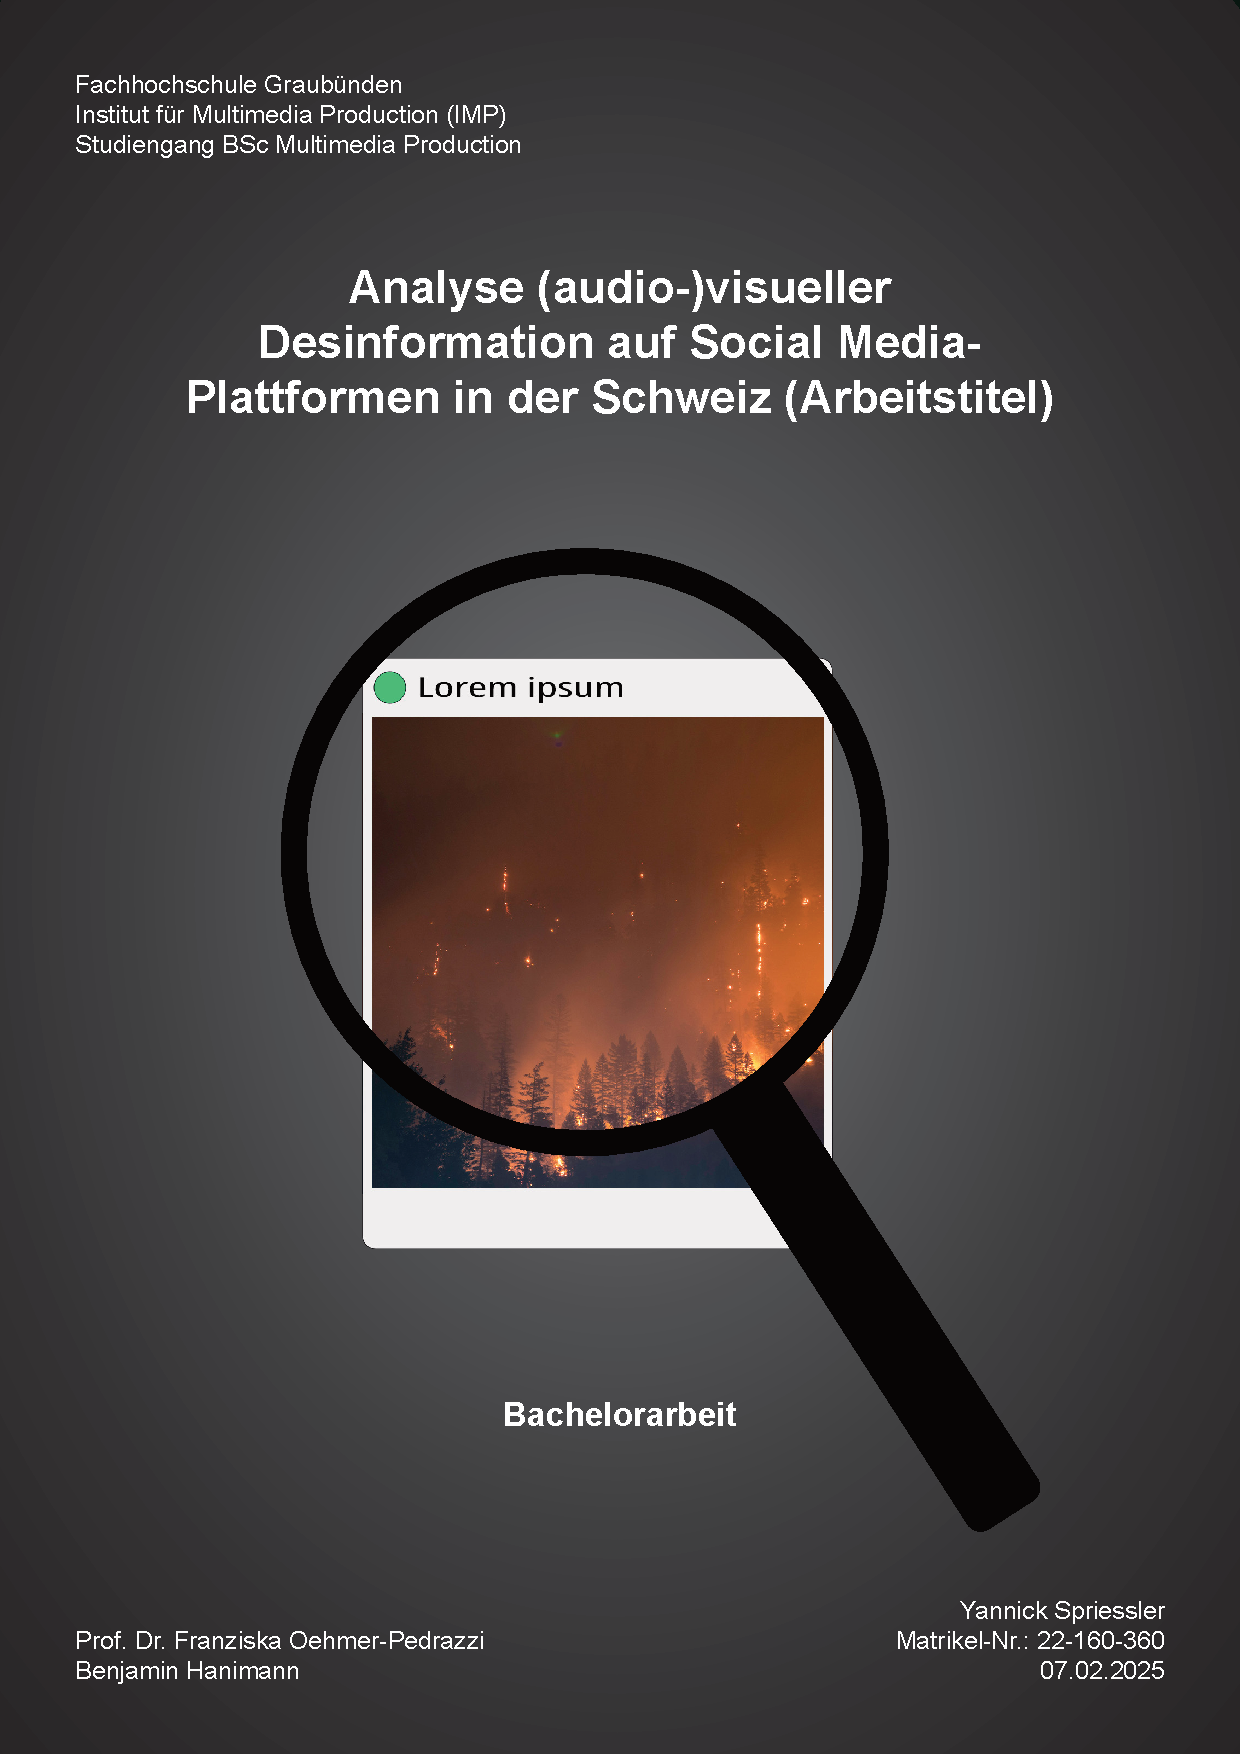
\includepdf{Titelblatt_Thesis}
  \nocite{howard_trees_2017}  %Citation for title page, only in image bibliography
\end{titlingpage}
\pagebreak      %Insert page break
%-----------------------------------------------
\renewcommand{\abstractname}{Abstract}
\begin{abstract}
  \setlength{\parindent}{0pt}
Die vorliegende Bachelorarbeit untersucht, welche Merkmale visuelle und audiovisuelle Desinformation auf Social-Media-Plattformen in der Schweiz aufweist. Hierfür wurde eine quantitative Inhaltsanalyse von durch Faktencheck-Plattformen als Desinformation deklarierten Beiträgen durchgeführt, welche anschliessend statistisch ausgewertet wurden.\\
Diese ergab, dass desinformierende Beiträge auf unterschiedlichen Plattformen geteilt werden, primär zu aktuellen Vorkommnissen. In Zusammenhang mit Bildern und Videos vermitteln sie die Desinformation auf emotionale Weise und können oft nur schwer als Desinformation erkannt werden.\\
Die Erkenntnisse aus der Thesis werden in Zusammenhang mit Experteninterviews verwendet, um eine interaktive Webplattform zur Aufklärung und Förderung der Medienkompetenz zu gestalten.
\\
\\
This bachelor's thesis analyses the specifications of visual and audiovisual disinformation on social media platforms in Switzerland. For this purpose, a quantitative content analysis of social media posts, labelled as disinformation by factchecking platforms, was performed and statistically analysed.\\
The results show that disinforming posts are shared on multiple social media platforms, especially concerning current events. Combined with images and videos, they provide the disinformation in an emotional way and can hardly be distinguished as disinformation.\\
The results of the thesis, combined with expert interviews, are used to create an interactive web platform to educate and strengthen media literacy.
\end{abstract}

\vfill
\textbf{Keywords:}\\ \textit{Audiovisuelle Desinformation, Social Media, Faktencheck, audiovisuelle Inhaltsanalyse, quantitative Inhaltsanalyse, Schweiz}

\textbf{Zitiervorschlag}:\\
\hangindent=2em
\hangafter=1
Spriessler, Y. (2025). \textit{(Audio-) visuelle Desinformation auf Social-Media-Plattformen in der Schweiz. Eine Analyse.} Bachelorarbeit. Chur: Fachhochschule Graubünden.

 \textbf{Titelblatt:}\\
Bild: \fullcite{howard_trees_2017}.\\
Titelblatt: Eigene Darstellung.
%\frontmatter   %If foreword
\pagebreak
%TOC
\thispagestyle{empty}
\setcounter{page}{0}    %Set page no.
\tableofcontents        %Content index
\pagebreak
%-----------------------------------------------
%DOC

%\mainmatter    %Main part if foreword used
\section{Einleitung}
Spätestens seit den US-Wahlen 2016 hat der Begriff «Fake News» stark an Bedeutung gewonnen. Zwar handelt es sich dabei nicht um eine Neuerscheinung und falsche Informationen wurden lange vor der Entwicklung des Internets verbreitet \parencites[214]{allcott_social_2017}[247]{hohlfeld_schlechte_2020}[1]{khan_fake_2021}, dennoch ist das Problem unter anderem durch die Verbreitung über das Internet weiter stark angewachsen \parencites[214–215]{allcott_social_2017}[1]{khan_fake_2021}[1]{lazer_science_2018}[4]{ceron_fake_2021}.\\
Aufgrund der sozialen Medien und der Möglichkeit, innerhalb kürzester Zeit Videos und Bilder zu produzieren, können heute sehr schnell audiovisuelle Falschinformationen verbreitet werden. Diese stellen nicht nur ein Problem für die individuellen Rezipierenden dar, sondern gefährden dabei auch politische und gesellschaftliche Prozesse.

Die Bachelorarbeit befasst sich damit, welche inhaltlichen und gestalterischen Merkmale audiovisuelle und bildbasierte Desinformation auf Social-Media-Plattformen in der Schweiz aufweist. \\
Ziel der Arbeit ist zum einen, herauszufinden, ob es mögliche Muster und Strategien hinter der Produktion der Inhalte gibt. Zum anderen soll auch ein allgemeines Verständnis über die entsprechenden Inhalte gewonnen werden. \\
Die Erkenntnisse der Bachelorarbeit werden anschliessend verwendet, um darauf basierend eine interaktive Aufklärungsplattform zu gestalten.

\subsection{Relevanz}
\textbf{Gesellschaft} \\
Im Jahr 2024 betrug der Anteil der Social-Media-Nutzenden in der Schweiz knapp 80 \%. Weiter informiert sich ein bedeutender Anteil der europäischen Bevölkerung über das Internet, eine Mehrheit verwendet Social Media primär für Nachrichten und Unterhaltung \parencite[21ff]{we_are_social_anteil_2024}. Gemäss der JAMES-Studie 2024 \parencite[40]{kulling-knecht_james_2024} informiert sich 2024 etwa die Hälfte der Jugendlichen täglich oder mehrmals pro Woche auf sozialen Plattformen. \\
Somit wird durch Social-Media-Inhalte ein Grossteil der Schweizer Bevölkerung erreicht. Dadurch können desinformierende Inhalte potenziell einen grossen Einfluss auf die Bevölkerung und ihre (politische) Meinungsbildung haben \parencites[18]{grujic_warnhinweise_2024}[258]{hohlfeld_schlechte_2020}[1f]{khan_fake_2021}, insbesondere wenn Social-Media-Plattformen auch als Informationsquelle zu politischen und gesellschaftlichen Themen dienen.

\textcite{grady_neural_1998} haben gezeigt, dass sich Rezipierende besser und länger an visuelle Inhalte erinnern können als an Worte. Eine weitere Untersuchung fand einen Zusammenhang zwischen dem Konsum von Videos und der Möglichkeit der Nutzenden, auf diese zu reagieren \parencite[242]{khan_social_2017}. Inhalte mit Partizipationsmöglichkeit scheinen ausserdem den weiteren Konsum (\textit{information seeking}) zu befeuern \parencite[243]{khan_social_2017}. \\
Insofern kann davon ausgegangen werden, dass audiovisuelle Desinformation eine besondere Gefahr darstellt.

\textbf{Politik} \\
\textcite[258]{hohlfeld_schlechte_2020} schreiben Desinformation die Fähigkeit zu, demokratische Gesellschaften \say{durch Inhalte, die Angst und Verunsicherung schüren, [\ldots] [sowie, d. Verf.] durch die Schwächung der seriösen Institutionen der Erkenntnisbeschaffung und [\ldots] durch Normverschiebungen des politisch Sagbaren} zu destabilisieren. \parencite[vgl.\ auch][1]{khan_fake_2021}.

Eine Marketingfirma fand 2016 heraus, dass Fake-News-Seiten für die Verbreitung ihrer Inhalte fast komplett  von Facebook abhängig sind. Während solche Seiten 50 \% der Websitebesuche von Facebook erhalten, lagen seriöse Medien bei etwa 20 \%.\parencites{wong_almost_2016}[zit.\ nach][1]{khan_fake_2021}[vgl.\ auch][212]{allcott_social_2017}. \\
Facebook und weitere Social-Media-Plattformen können somit als starke Treiber von Desinformation verstanden werden \parencite{wong_almost_2016}. In Anbetracht der jüngsten Tendenz, Einordnungen durch Faktencheck-Organisationen auf den Meta-Plattformen einzustellen \parencites{isaac_meta_2025}{meta_transparency_centre_penalties_2025}, ist es für die Nutzenden deshalb umso wichtiger, Inhalte bezüglich ihres Wahrheitsgehalts korrekt einordnen zu können.

Gemäss dem \textcites{bundesministerium_des_innern_und_fur_heimat_desinformation_2022}\parencite[zit.\ nach][15]{teetz_social-media-post_2023} kann Desinformation in einigen Fällen sogar als Bedrohung der nationalen Sicherheit verstanden werden. \\
Die Schweiz hat mit ihrer direkten Demokratie ein weltweit einzigartiges politisches System, in keinem anderen Staat hat die Bevölkerung so viele Mitbestimmungsrechte \parencite[2]{sager_politische_2017}. Es ist deshalb zwingend notwendig, dass diese ihre politischen Entscheide aufgrund von korrekten Fakten und eigener politischer Entscheidung treffen kann, ohne von Desinformation beeinflusst zu werden \parencite[26]{vogler_wahrnehmung_2021}\parencite[vgl.\ auch][14f]{european_parliament_directorate-general_for_external_policies_of_the_union_impact_2021}. Auch wenn über die tatsächliche Gefährdung der Schweizer Politik durch Desinformation bisher noch wenig bekannt ist, scheint die Schweiz als Staat vergleichsweise widerstandsfähig zu sein (ebd.).\\
Durch das Wissen der Plattform-Nutzenden über Desinformation und die Mechanismen der Social-Media-Plattformen sowie die Fähigkeit, falsche von echten Tatsachen zu unterscheiden, kann diese Gefahr weiter verringert werden.

\textbf{Wissenschaft} \\
Soziale Medien funktionieren fundamental anders als traditionelle Medien. Nachrichten und andere Inhalte können ohne faktische Einordnung oder inhaltlichen Kodex weltweit geteilt werden \parencite[211]{allcott_social_2017}. Die journalistischen Kriterien wie \say{Unabhängigkeit,  Ausgewogenheit, Vielfalt, Verständlichkeit und Unterhaltsamkeit}\parencite[9]{grujic_warnhinweise_2024} werden nicht überprüft. Besonders in Krisenzeiten sind die Nutzenden besonders anfällig für Falschinformationen \parencite[vgl.][2]{ceron_fake_2021}. \\
Social-Media-Plattformen und ihre entsprechenden Algorithmen zur Inhaltsauswahl basieren neben den Interaktionen der Nutzenden untereinander in ihrer Funktionsweise vor allem auf der Generierung von Aufmerksamkeit \parencites[vgl.][220]{schmidt_meinungsbildung_2022}[493]{behnke_manipulation_2018}. \\
Durch die Verbreitung eines Inhaltes wird zwangsläufig die Kapazität der Nutzenden für die Verarbeitung anderer Inhalte geschmälert \parencite[248]{hohlfeld_schlechte_2020}.

Die Wissenschaft kennt das Potenzial und die Gefahr von Social-Media-Plattformen, durch Fragmentierung und das Anzeigen bestimmter Inhalte Filterblasen zu schaffen und die Gesellschaft zu spalten – dieser Effekt konnte jedoch bisher nicht tatsächlich bewiesen werden \parencite[220]{schmidt_meinungsbildung_2022}.

Als Massnahme gegen Desinformation werden oft Faktenchecks eingesetzt. Deren Wirksamkeit wird allerdings immer wieder in Frage gestellt \parencites[1095]{lazer_science_2018}[4f]{ceron_fake_2021}. \say{(\ldots) people prefer information that confirms their preexisting attitudes (selective exposure), view information consistent with their preexisting beliefs as more persuasive than dissonant information (confirmation bias), and are inclined to accept information that pleases them (desirability bias).} \parencites[1095]{lazer_science_2018}\parencite[vgl.\ auch][18]{grujic_warnhinweise_2024}. Faktenchecks könnten in einigen Fällen sogar kontraproduktiv sein, wenn  die Falschinformation wieder aufgefrischt wird und dadurch eher hängenbleibt als die faktische Einordnung (ebd.). Umso wichtiger ist es, dass die Rezipierenden die medialen Artefakte möglichst selbst beurteilen können.

\subsection{Forschungsfrage}
\label{thesis}
Folgende Fragestellung wird in der Bachelorarbeit behandelt:
\begin{quote}
  Welche inhaltlichen und gestalterischen Merkmale weist visuelle und audiovisuelle Desinformation auf Social-Media-Plattformen in der Schweiz auf?
\end{quote}
Desinformation kann gravierende Folgen für eine Gesellschaft haben.
Aufgrund der Relevanz von Social-Media-Plattformen für die individuelle Informationsbeschaffung in der heutigen Zeit ist es unabdingbar, ein Verständnis über die Mechanismen zu erlangen, mit welchen Desinformation arbeitet, um die Rezipierenden zu täuschen. So kann nicht nur die eigene Medienkompetenz gestärkt werden, Desinformation zu erkennen, sondern deren Schadenspotenzial kann optimalerweise zusätzlich eingedämmt werden.

Gemäss der Einordnung nach \cite[37]{lasswell_lasswell_1948} bewegt sich diese Arbeit im Bereich der Inhalts- und Kanalforschung. Es wird untersucht, durch wen Desinformation verbreitet wird und welche Merkmale diese aufweist.

\label{structure}
Im Kapitel \ref{sec:theory} \nameref{sec:theory} wird hierfür der aktuelle Forschungsstand dargelegt. Nach einer Begriffsdefinition folgt eine Übersicht über die aktuellen Erkenntnisse zur Verbreitung und Produktion von desinformierenden Inhalten. \\
Kapitel \ref{sec:method} \nameref{sec:method} widmet sich der angewandten Methode und mündet in den \nameref{sec:results}n in Kapitel \ref{sec:results}.

\pagebreak
\section{Forschungsstand zur Desinformation}
\label{sec:theory}
Das folgende Kapitel fasst den aktuellen Forschungsstand zu aktueller Desinformation zusammen. Während Desinformation auch in Printmedien wie Zeitungen oder Fernsehformaten verbreitet werden kann, konzentriert sich diese Arbeit auf die Verbreitung von Desinformation auf Social-Media-Plattformen.\\
In einem ersten Schritt wird aktuelle Desinformation definiert und von anderen, ähnlichen Formaten abgegrenzt. Anschliessend wird das Phänomen erklärt, indem auf die Verbreitung und die inhaltliche und strukturelle Produktion sowie die Auswirkungen davon eingegangen wird. \\
Dazu werden aktuelle Studien aufgearbeitet und die entsprechenden Erkenntnisse gesammelt dargestellt.

\subsection{Begriffsdefinition}
\label{theory_definition}
Beispielsweise durch die erste Amtszeit des US-Präsidenten Donald Trump (2017–2021) oder den Brexit hat der Begriff «Fake News» weltweit an Bedeutung gewonnen \parencites[1f]{hohlfeld_schlechte_2020}[1]{marx_fake_2020}. \\
In der Literatur existieren verschiedene Definitionen des Begriffes. \textcite[246f]{hohlfeld_schlechte_2020} vertreten beispielsweise die Haltung, dass «Fake News» als Begriff für desinformierende Inhalte gleichbedeutend sind mit dem politischen Propagandabegriff. In den letzten Jahren wurde allerdings auch oft argumentiert, dass «Fake News» lediglich als politischer Begriff gewertet und im wissenschaftlichen Kontext stattdessen von (aktueller) Desinformation gesprochen werden sollte \parencites[3]{bontridder_role_2021}{habgood-coote_stop_2019}[148]{marx_fake_2020}. Egelhofer \& Lecheler \parencite[zit.\ nach][148]{marx_fake_2020} differenzieren zwischen «Fake News» als Genre für Falschinformationen und «Fake News» als Label im Sinne einer politischen Instrumentalisierung zur Diskreditierung von Medien und Institutionen.\\
In Anlehnung an \textcite{marx_fake_2020} und in Abgrenzung zum politischen Label wird in dieser Bachelorarbeit der Begriff «Desinformation» verwendet.

In der Wissenschaft gibt es bisher keine einstimmige Definition für Desinformation.
\textcite[148f]{marx_fake_2020} benennen ein Theoriendefizit, basierend auf widersprüchlichen Definitionen sowie nicht nachvollziehbaren Definitionskriterien.\\
Laut \textcite[1094]{lazer_science_2018} handelt es sich bei Desinformation um \say{fabricated information that mimics news media content in form but not in organizational process or intent. Fake-news outlets, in turn, lack the news media’s editorial norms and processes for ensuring the accuracy and credibility of information.}
\textcite[213]{allcott_social_2017} sprechen von \say{(\ldots) news articles that are intentionally and verifiably false, and could mislead readers.} \parencites[vgl.\ auch][140]{tandoc_jr_defining_2018}[1094]{lazer_science_2018}.\\
Diese Definition kann nicht nur auf News-Artikel angewendet werden, sondern auch auf andere mediale Artefakte \parencite[3]{bontridder_role_2021} \parencite[vgl.\ auch][16]{reuter_fake_2019}. \textcite[1]{marx_fake_2020} definieren aktuelle Desinformation als \say{Kommunikation wissentlich und empirisch falscher Informationen zu neuen und relevanten Sachverhalten mit dem Anspruch auf Wahrheit.} Sie stützen sich dabei auf folgende Kriterien:

\begin{itemize}
  \item \textbf{(Visuelle) Kommunikation}: Eine wahrheitsfähige Mitteilung mit darstellendem Gehalt, welche einen Teil der Wirklichkeit abbildet. Dies bezieht sich nicht nur auf sprachliche, sondern auch auf visuelle Mitteilungen \parencite[151]{marx_fake_2020}.
  \item \textbf{Aktualitätsbezug}: \say{(\ldots) überraschende Themen mit (potenziell) großer Auswirkung auf die Gesellschaft. So ermöglicht sie ihrem Publikum die Ausbildung von (wenn auch empirisch unzutreffenden [\ldots]) Erwartungen und dadurch die Orientierung in einer komplexen Welt.} \parencite[152]{marx_fake_2020}.
  \item \textbf{Wahrheitsanspruch}: Aktuelle Desinformation beansprucht für sich, dass sie (vorgetäuscht) wahr ist. In diese Betrachtung werden sowohl Produzierende wie auch Rezipierende des Inhaltes miteinbezogen. Hierbei gilt, ob es für externe Beobachtende plausibel ist, dass Rezipierende die Nachricht als wahr betrachten \parencite[153]{marx_fake_2020}.
  \item \textbf{Unwahrheit}: Der desinformierende Inhalt besitzt irreführendes Potenzial, da er empirisch falsch ist und somit den zuvor beanspruchten Wahrheitsgehalt nicht einlöst. \parencite[154]{marx_fake_2020}.
  \item \textbf{Unwahrhaftigkeit}: Die Produzierenden sind sich der Tatsache bewusst, dass ihre Mitteilungen falsch sind. \parencite[156]{marx_fake_2020}
  \item \textbf{Täuschungsabsicht}: Falsche Tatsachen werden vorsätzlich und bewusst verbreitet. Dabei spielt es keine Rolle, ob diese der gezielten Verbreitung von Falschinformationen dienen sollen oder beispielsweise zu Clickbait-Zwecken eingesetzt werden \parencites[157]{marx_fake_2020}[vgl.\ auch][2]{khan_fake_2021}.
\end{itemize}

Desinformation muss abgegrenzt werden von weiteren verwandten Themen und Begriffen:
\begin{itemize}
  \item \textbf{Missinformation}: Missinformation \say{ (\ldots) refers to false, inaccurate, or misleading information that is shared without any intent to deceive.} \parencite[2]{bontridder_role_2021}. \citeauthor{marx_fake_2020} grenzen Missinformation anhand des Unwahrhaftigkeitskriteriums ab, indem es sich bei Missinformation gemäss ihrer Definition um eine unwissentliche Fehlinformation handelt \parencite[156]{marx_fake_2020}, welche ohne Täuschungsabsicht verbreitet wird \parencite[vgl.\ auch][15]{grujic_warnhinweise_2024}.
  \item \textbf{Satire}: Satire ist nach \textcite[154]{marx_fake_2020} erkennbar an einer klaren Quelle (beispielsweise ein Satiremagazin) sowie bestimmten Text- und Stilmerkmalen und grenzt sich von Desinformation ab durch den Verzicht auf den Wahrheitsanspruch. Diese Einschätzung wird ebenfalls durch externe Beobachtende getroffen.\\
    Weitere Merkmale sind humoristische oder übertriebene Darstellungen \parencites[141]{tandoc_jr_defining_2018}[2]{khan_fake_2021}, obwohl diese auch in seriösen und korrekten Nachrichten verwendet werden können.
  \item \textbf{Gerücht}: Ein Gerücht zeichnet sich dadurch aus, dass sein Wahrheitsgehalt (noch) nicht überprüft ist \parencite[155]{marx_fake_2020}. Der Wahrheitsgehalt von Desinformation lässt sich jederzeit prüfen.
  \item \textbf{Verschwörungstheorie}: Rosnow \& Kimmel \parencite[zit.\ nach][197]{krafft_disinformation_2020} definieren Verschwörungstheorien (Rumors) als \say{an unverified proposition for belief that bears topical relevance for persons actively involved in its dissemination.} (ebd.). \textcite[197]{krafft_disinformation_2020} halten eine persönliche Betroffenheit sowie Informationsunsicherheit als Bedingungen für eine Verschwörungstheorie fest.\\
    Von Desinformation unterscheidet sich eine Verschwörungstheorie dadurch, dass sie meist auch von denjenigen geglaubt wird, welche zu ihrer Verbreitung beitragen \parencite[156]{marx_fake_2020}.
  \item \textbf{Fake News}: Zum einen wird der Begriff im politischen Kontext als abwertendes Label verwendet für Nachrichten, welche nicht nach dem Willen der politischen Akteurinnen und Akteure berichten \parencite[3]{tandoc_jr_facts_2019}.\\
    Zum anderen handelt es sich bei «Fake News» um eine Unterkategorie der Desinformation, welche spezifisch Nachrichtenartikel bezeichnet, die Falschinformationen beinhalten und so aufbereitet sind, dass sie für echt gehalten werden (können) (ebd.).
\end{itemize}

\citeauthor{marx_fake_2020} haben in ihrer Arbeit eine Begriffsdefinition für aktuelle Desinformation aufgestellt, welche den Term klar definiert und von anderen Kategorien von Falschinformationen abgrenzt. In dieser Bachelorarbeit wird nachfolgend ihre Definition zur Beurteilung von Desinformation angesetzt.
\subsubsection{Was aktuelle Desinformation ist}
Viele Publikationen halten fest, dass aktuelle Desinformation kein neues Phänomen ist \parencites[vgl.\ bspw.][2]{tandoc_jr_facts_2019}[214]{allcott_social_2017}[1094]{lazer_science_2018}. \textcite[214]{allcott_social_2017} nennen als eines der ältesten Beispiele den \textit{Great Moon Hoax} von 1835.

\subsection{Studien zu aktueller Desinformation}
Seit in den letzten 20 Jahren Social-Media-Plattformen aufgekommen sind, hat sich die traditionelle Informationsverbreitung stark ins Internet verlagert \parencites[211]{allcott_social_2017}[147]{marx_fake_2020}[138]{tandoc_jr_defining_2018}[1094]{lazer_science_2018}. Diese Plattformen erlauben es den Nutzenden, auf sehr einfache Art und ohne grosse Hindernisse Informationen online mit der gesamten Nutzerbasis zu teilen \parencites[1]{vogler_wahrnehmung_2021}{lazer_science_2018}. Informationen zu aktuellen Ereignissen können so ohne inhaltliche Richtlinien, Einordnungen oder Faktenkontrollen potenziell weltweit verbreitet werden \parencites[147]{marx_fake_2020}[211]{allcott_social_2017}[4]{ceron_fake_2021}[165f]{wahl_fake_2021}. \say{An individual user with no track record or reputation can in some cases reach as many readers as Fox News, CNN, or the New York Times.} \parencite[211]{allcott_social_2017}.

Mittlerweile informiert sich weltweit ein Grossteil der Bevölkerung auf sozialen Plattformen oder anderweitig online über aktuelle Geschehnisse \parencite[212]{allcott_social_2017}. Auch in der Schweiz nutzt mehr als die Hälfte der Bevölkerung soziale Medien zu Unterhaltungs- und Informationszwecken \parencite[21ff]{we_are_social_anteil_2024}. Nutzende, welche auf Social Media Inhalte zu aktuellen Vorkommnissen teilen, werden so journalistisch tätig, auch ohne sich dessen immer bewusst zu sein \parencite[139]{tandoc_jr_defining_2018}. Professionelle Journalisten und Medienhäuser sind diesem Trend in den letzten Jahren gefolgt und nutzen die Plattformen mittlerweile ebenfalls gezielt zur Verbreitung ihrer Inhalte (ebd.).

Die grosse Freiheit, welche diese Liberalisierung der Inhaltsverbreitung bietet, lässt gleichzeitig Raum für Missbrauch und die Verbreitung von Falschinformationen \parencite[4]{ceron_fake_2021}.\\
Seit 2016 ist vor allem in den USA das Mass an Desinformation stark angestiegen, bedingt durch den Wahlkampf von US-Präsident Donald Trump \parencites[1094f]{lazer_science_2018}{allcott_social_2017}[147]{marx_fake_2020}[147]{tandoc_jr_defining_2018}. \textcite[1094f]{lazer_science_2018} konstatieren einen historischen Tiefpunkt in der Glaubwürdigkeit in die öffentlichen Medien. Durch parteipolitische Polarisierung und geringere Toleranz für andere Meinungen durch Social-Media-Inhalte ist ein massiver Nährboden entstanden für die Verbreitung von Desinformation (ebd.).\\
Während der Covid-Pandemie 2020 wurde ebenfalls ein starker Anstieg an Desinformation auf den sozialen Medien verzeichnet, beispielsweise zu den neu entwickelten Impfstoffen \parencite[2]{khan_fake_2021}. \Textcite[2]{ceron_fake_2021} nennen als Ursache die vorherrschende Unsicherheit, welche die Verbreitung der Inhalte weiter befeuerte \parencite[vgl.\ auch][22f]{zoglauer_konstruierte_2021}. \\

Die Schweiz galt lange als vergleichsweise resistent gegen Desinformation \parencite[26]{vogler_wahrnehmung_2021}. Jedoch lässt sich auch hier seit 2021 ein Anstieg verzeichnen. Für die Schweiz gaben 2021 etwa ein Viertel der befragten Personen an, oft oder sehr oft auf Desinformation zu stossen (ebd.). In einer OECD-Studie von 2024 zeigte sich ausserdem, dass die Schweizer Bevölkerung in der Bewertung von Desinformation vergleichsweise schlecht abschnitt \parencite{wyl_schweizerinnen_2024}.

\subsubsection{Wer verbreitet Desinformation?}
~\label{theory_disseminents}
% Ursprung
Die meisten Bürgerinnen und Bürger moderner Demokratien informieren sich nicht selbst aktiv über Themen wie Politik und die Gesellschaft, sondern ihr Wissensstand ist abhängig von den zur Verfügung stehenden Informationen der \say{information supply chain} \parencite[69]{lecheler_disinformation_2022}. Diese wird bespielt mit journalistisch oder anderweitig medial aufbereiteten Inhalten, welche von den leitenden Akteurinnen und Akteuren der Gesellschaft ausgehen (ebd.). Gemäss \textcite[217]{allcott_social_2017} stammen die Inhalte ursprünglich oftmals von Desinformations- oder Satire-Plattformen und werden von da aus weiterverbreitet.

% generelle Motivation hinter der Verbreitung
Da die Produktion von Desinformation einen bewussten Akt der Täuschung darstellt, kann davon ausgegangen werden, dass es schwierig ist, tatsächliche Aussagen über die Produzierenden zu treffen \parencite[73]{lecheler_disinformation_2022}. \textcite[39]{pennycook_lazy_2019} benennen als Grundmotivation jedoch bereits in ihrer Definition von Desinformation \say{highly salient [\ldots] fabricated claims that are created to spread on social media.} Die Literatur nennt zumeist zwei klare Motive zur Produktion von Desinformation: finanzielle Anreize oder politische und ideologische Überlegungen.

Gehen Inhalte auf Social Media viral und werden einer grossen Menge an Nutzenden angezeigt, so generiert dies oft finanziellen Umsatz \parencites[217]{allcott_social_2017}[3]{tandoc_jr_facts_2019}[157]{marx_fake_2020}, indem beispielsweise auf externe Artikel verlinkt wird, welche dann Werbeanzeigen beinhalten. \textcite[76]{lecheler_disinformation_2022} weisen hier etwa auf Journalistinnen und Journalisten oder Medienhäuser hin, welche bewusst desinformierende Taktiken einsetzen, um durch Clickbaiting oder besonders polarisierende Inhalte mehr Umsatz zu generieren. \\
Doch nicht nur journalistische Akteurinnen und Akteure verwenden Desinformation aus finanziellen Gründen, sondern auch Privatpersonen. Ein berühmtes Beispiel stammt von den US-Wahlen 2016, als eine Gruppe Jugendlicher in Mazedonien massenweise Desinformation verbreitet hat, was ihnen Tausende von Dollars einbrachte \parencites[217]{allcott_social_2017}[vgl.\ auch][]{subramanian_meet_2017}[3]{tandoc_jr_facts_2019}. \textcite[217]{allcott_social_2017} erwähnen als weiteres Beispiel Paul Horner, welcher aus Profitgründen massenweise Desinformation auf Social Media geteilt hat \parencite[vgl.\ auch][]{dewey_facebook_2016}.

Als zweiter Motivationstreiber gelten ideologisch motivierte Versuche, Einfluss auf die politische Meinungsbildung zu nehmen und demokratische Institutionen zu schwächen \parencites[225]{schmidt_meinungsbildung_2022}[75]{lecheler_disinformation_2022}[157]{marx_fake_2020}. So werden zum Beispiel oftmals Politikerinnen und Politiker diskreditiert \parencites[3]{tandoc_jr_facts_2019}[217]{allcott_social_2017} oder bewusst polarisierende Inhalte verbreitet \parencites[8]{european_parliament_directorate-general_for_external_policies_of_the_union_impact_2021}[3]{tandoc_jr_facts_2019}.\\
Ergänzend halten \textcite[182]{weidner_fake_2019} fest, dass Einzelpersonen oder feindliche Staaten diskreditierende oder anderweitig politische Desinformation weniger gezielt einsetzen, sondern allgemeiner nach dem Motto \say{I’d like to see your world burn}. Das Ziel dahinter ist auch hier die Delegitimierung eines staatlichen Systems sowie eine Spaltung der Gesellschaft (ebd.)

% Weiterverbreitung durch Nutzende
Laut \textcite[3]{tandoc_jr_facts_2019} lassen sich Produzierende meist von den Nutzenden unterscheiden, welche die Desinformation weiterverbreiten. Dies unterstreichen auch \textcite[77]{lecheler_disinformation_2022}: oftmals verfolgen die Rezipierenden mit der Weiterleitung der Inhalte nicht das Ziel, demokratische Institutionen zu schwächen, sondern wollen entweder ihr Umfeld informieren oder unterhalten \parencite[bspw.]{subramanian_meet_2017}, oder aber sie glauben die Desinformation selbst. Die Information wird in diesem Fall entweder geteilt, um beispielsweise eine hoffnungsvolle Botschaft zu verbreiten, oder um das Umfeld zu warnen \parencite[182]{weidner_fake_2019}. Unabhängig vom tatsächlichen Grund tragen sie durch das Weiterleiten des Inhalts jedoch zur Verbreitung der Desinformation bei.\\
\textcite[2]{guess_less_2019} zeigen ausserdem, dass die Nutzenden, welche besonders viele Links teilen, oftmals auch besser zwischen wahren und falschen Informationen unterscheiden können. Es ist also nicht der Fall, dass einige Nutzende einfach blindlings alles teilen (ebd.).

\subsubsection{Die Produktion von Desinformation}
~\label{theory_production}
% Psychologische Faktoren, weshalb Desinformation funktioniert
Auf der Produktionsseite werden oftmals psychologische Faktoren ausgenutzt, um die Desinformation gezielt zu verbreiten: Es wird darauf gesetzt, dass Rezipierende \say{attracted to gossip, rumor, scandal, innuendo, and the unlikely} sind \parencite[8]{burkhardt_history_2017}. Desinformation wird besonders emotional und provokativ gestaltet, beispielsweise durch Enthusiasmus, Wut oder Enttäuschung, um so möglichst viel Aufmerksamkeit auf sich zu ziehen \parencites[42]{levak_disinformation_2020}[18]{grujic_warnhinweise_2024}[5]{tandoc_jr_facts_2019}[170]{wahl_fake_2021}. Durch ihre Aufbereitungsart wird den Rezipierenden Orientierung geboten und Erwartungen werden geschürt, auch wenn diese empirisch nicht zutreffen \parencite[152]{marx_fake_2020}. \\
\textcite[45]{pennycook_lazy_2019} weisen darauf hin, dass durch diesen Fokus auf Viralität oftmals die Plausibilität der Nachrichten sinkt, weshalb eher analytisch denkende Personen tendenziell weniger anfällig für Desinformation sein könnten (siehe Kapitel~\say{\ref{theory_credibility}~\nameref{theory_credibility}}).

% Technisch / Produktion / Inhalt
Um glaubhaft zu sein, muss Desinformation immer noch genügend Wahrheitsgehalt haben, um genug wahr zu erscheinen, auch wenn sie faktisch falsch ist. \parencite[Pennycook et al. (2018), zit\ nach][182]{weidner_fake_2019}. \\
Viele Quellen belegen, dass Desinformation oft an echte Nachrichtenformate angelehnt ist, um so möglichst für echt gehalten zu werden \parencites[3]{tandoc_jr_facts_2019}[213]{allcott_social_2017}[1094]{lazer_science_2018}[10f]{grujic_warnhinweise_2024}. \textcite[15]{grujic_warnhinweise_2024} benennt weitere typische Merkmale, wie beispielsweise reisserische Überschriften oder fehlende Quellenangaben. Studien zeigen ausserdem, dass visuelle Artefakte in Kombination mit Text weiter zur Aufmerksamkeit für die Desinformation beitragen \parencites[3701]{weikmann_visual_2023}[182]{weidner_fake_2019}. Das Kapitel~\say{\ref{theory_audiovisual_content}~\nameref{theory_audiovisual_content}} geht weiter auf die visuelle Wirkung von Desinformation ein.

\textbf{Verbreitung}\\
~\label{theory_distribution}
Digitale Social-Media-Plattformen ermöglichen es sämtlichen Nutzenden, Informationen einem nahezu unbegrenzten Publikum zugänglich zu machen \parencite[147]{marx_fake_2020}. \textcite[485]{schaewitz_when_2020} stellen dazu klar, dass negative Auswirkungen von Desinformation nur dann zu erwarten sind, wenn diese nach Prüfung durch die Rezipierenden geglaubt und weiterverbreitet wird. Eine Information, welche von Anfang an nicht glaubwürdig ist, wird in den wenigsten Fällen weiterverbreitet, es sei denn mit mutwilliger Absicht. \textcite{guess_less_2019} zeigen, dass die Weiterverbreitung von Desinformation durch Rezipierende generell eher selten stattfindet.

Wird ein desinformierender Inhalt auf Social Media weiterverbreitet, geschieht die Distribution nicht nur durch die Nutzenden selbst, sondern wird durch die Funktionsweise der Plattformen weiter vorangetrieben \parencite[vgl.\ auch][199]{krafft_disinformation_2020}.
Was die Verbreitung auf Social Media so effektiv macht, ist die Personalisierung der Inhalte basierend auf den Plattform-Algorithmen \parencite[219f]{schmidt_meinungsbildung_2022}: Um die Nutzenden möglichst lange auf den Plattformen zu halten, werden ihnen gezielt Inhalte angezeigt, welche sie ansprechen und ihre Aufmerksamkeit erhalten. Dadurch wird Desinformation gezielt vor allem denjenigen Personen angezeigt, welche diese mit hoher Wahrscheinlichkeit weiter teilen und so weitere Aufmerksamkeit generieren. Während die Plattformen so mehr Einnahmen durch angezeigte Werbung machen, führt es dazu, dass sich Desinformation weiter verbreiten kann (ebd.) \parencite[vgl.\ auch][967]{ghai_deep-learning-based_2024}.

Ausserdem kursieren auf den sozialen Plattformen sogenannte \textit{Bots}.
\begin{quote}
  Der Obergriff  \textit{social bots} oder deren Zusammenschluss zu einem \textit{social botnet} beschreibt auf Algorithmen basierende maschinelle Nutzer, die vollautomatisiert konkrete Aufgaben in digitalen sozialen Netzwerken abarbeiten und dabei weitgehend autark agieren. So können social bots inzwischen mit menschlichen Nutzerinnen und Nutzern interagieren und kommunizieren, Gesprächen folgen und dem Kontext entsprechende Kommentare erwidern[\ldots]. \parencite[493f]{behnke_manipulation_2018}
\end{quote}
Bots nehmen Einfluss auf die Verbreitung von Inhalten oder Diskussionsverläufen (beispielsweise auf X/Twitter) und können so bestimmte Meinungen und Inhalte auf den Plattformen gezielt vorantreiben \parencite[495f]{behnke_manipulation_2018}. Da Bots oft nur sehr schwer oder gar nicht von echten Profilen zu unterscheiden sind, muss davon ausgegangen werden, dass eine Grosszahl der eingesetzten Bots nicht als solche erkannt wird \parencite[1095]{lazer_science_2018}.

\subsubsection{Glaubwürdigkeit von Desinformation}
~\label{theory_credibility}
Erkenntnisse zur Anfälligkeit der Rezipierenden, Desinformation zu glauben, und den entsprechenden Faktoren, welche dies begünstigen, sind weiterhin Gegenstand der Forschung \parencites[1094]{lazer_science_2018}[486]{schaewitz_when_2020}. Dennoch sind in der Wissenschaft bereits einige Theorien bekannt:

\textcite[248]{hohlfeld_schlechte_2020} erwähnen als ein Gefahrenpotenzial die limitierte kognitive Informationsverarbeitung, welche durch die Menge an über das Internet zugänglichen Informationen überschritten wird, insbesondere auf Social Media. So findet zwangsläufig eine inhaltliche Selektion der Inhalte statt, auf welche die Aufmerksamkeit verteilt werden muss (ebd.) \parencite[vgl.\ auch][5]{tandoc_jr_facts_2019}. Kommen Nutzende zu einem grossen Teil mit Desinformation in Kontakt, erscheint diese als glaubwürdiger und gewinnt an Relevanz, da weniger gedankliche Kapazität für andere Themen vorhanden ist.

In diesem Zusammenhang wird oft auf die \textit{dual-process theory} hingewiesen, gemäss der Informationen im Gehirn auf zwei Arten verarbeitet werden können \parencite[40]{pennycook_lazy_2019}: Während System 1 für intuitive, schnelle und automatische Entscheidungen verantwortlich ist, ermöglicht System 2 kalkulierende, analytische und bewusste Denkprozesse \parencite[249]{hohlfeld_schlechte_2020}. Gemäss \textcite[487]{schaewitz_when_2020} steigt durch Informationsüberfluss die Tendenz, Information intuitiv zu verarbeiten, da so trotz limitierter kognitiver Kapazität besser mit der übermässigen Menge an Inhalten umgegangen werden kann.
Eine Studie von \textcite[48]{pennycook_lazy_2019} belegt, dass Inhalte auf sozialen Medien tatsächlich zumeist heuristisch verarbeitet werden und Personen anfälliger sind für Desinformation, wenn sie Inhalte nach diesem intuitiven System beurteilen. Als Ursache hierfür beschreiben sie die meist fehlende Bereitschaft, sich vertiefter mit den Inhalten auseinanderzusetzen (ebd.). Das hat einen Einfluss auf die Fähigkeit zur Meinungsbildung, da diese ein aktives Mitdenken und Handeln erfordert \parencite[216]{schmidt_meinungsbildung_2022}. Fehlt diese vertiefte Auseinandersetzung, werden Inhalte einerseits schneller geglaubt, andererseits möglicherweise auch eher gedankenlos weiterverbreitet.

Während \citeauthor{pennycook_lazy_2019} also zum Schluss kommen, dass vor allem die Bereitschaft zur analytischen Beurteilung von Inhalten die Anfälligkeit für Desinformation beeinflusst und die politische Zugehörigkeit eine untergeordnete Rolle spielt, war das Ergebnis von \textcite[502]{schaewitz_when_2020} im Gegenzug, dass politische Zugehörigkeit sowie persönliche inhaltliche Bindung (\textit{motivated reasoning}) bei Versuchspersonen dennoch zumindest in gewissen Fällen eine grössere Rolle bezüglich der Vulnerabilität spielt als die Art der Informationsverarbeitung. \\
\textcite[24]{zoglauer_konstruierte_2021} argumentiert, dass aufgrund von persönlichen Stereotypen beide Faktoren einen Einfluss haben können und sich gegenseitig nicht zwingend ausschliessen müssen, respektive diese gemeinsam auftreten können.

Die Literatur kennt verschiedene Arten von Biases. \textcite{lazer_science_2018} nennen im Zusammenhang mit Desinformation die Folgenden:
\begin{itemize}
  \item{Selective exposure}: Rezipierende bevorzugen Informationen, die ihre bereits existierenden Einstellungen abbilden oder bestätigen.
  \item{Confirmation bias}: Information, welche mit bereits bestehenden Einstellungen übereinstimmt, wird als überzeugender wahrgenommen.
  \item{Desirability bias}: Rezipierende mögen Informationen mehr, wenn sie mit ihren Einstellungen übereinstimmen.
\end{itemize}
Von Biases wird angenommen, dass sie die Verarbeitung von Informationen vereinfachen, was jedoch weiter in einer erhöhten Angriffsfläche für Desinformation resultiert \parencite[5]{tandoc_jr_facts_2019}.  \textcite[1095]{lazer_science_2018} zweifeln basierend darauf die Effizienz von Faktenchecks an. Sie sehen ausserdem eine zusätzliche Gefahr darin, dass Personen durch Faktenchecks an bereits bekannte Informationen erinnert werden, diese durch ihre Biases aber im falschen Kontext abgespeichert werden und sich die Falschinformationen dadurch weiter festsetzen können (ebd.). \textcite[250]{hohlfeld_schlechte_2020} ergänzen, dass ein Bias (spezifisch vor allem der Bestätigungsfehler, \textit{confirmation bias}) oft auch dazu führt, dass Informationen weniger überprüft werden. Er führe dadurch auch eher zur Tendenz, sich in sogenannten Resonanzräumen zu organisieren.

Resonanzräume oder Echokammern bezeichnen den Umstand, dass sich Nutzende bewusst primär mit Gleichdenkenden umgeben. Dadurch werden sie weniger mit anderen Meinungen konfrontiert, welche nicht ihren eigenen entsprechen, wodurch sie in ihren (möglicherweise faktisch falschen) Vorstellungen bestätigt werden \parencites[250]{hohlfeld_schlechte_2020}[vgl.\ auch][8]{zoglauer_konstruierte_2021}[222]{schmidt_meinungsbildung_2022}[195]{krafft_disinformation_2020}[8]{grujic_warnhinweise_2024}[221]{allcott_social_2017}. \textcite[139]{tandoc_jr_defining_2018} zeigt ausserdem, dass Informationen von sozial näheren Quellen generell als wahrer wahrgenommen werden \parencite[vgl.\ auch][42]{levak_disinformation_2020}. \\
Von Echokammern wird befürchtet, dass sie zur gesellschaftlichen Spaltung und Polarisierung beitragen \parencite[8]{zoglauer_konstruierte_2021} und so die demokratische Meinungsbildung gefährden können, allerdings wird ihre Verbreitung und das Ausmass davon zunehmend infrage gestellt \parencite[222]{schmidt_meinungsbildung_2022}.

Gemäss \textcite[183]{weidner_fake_2019} ist vielen Nutzenden bekannt, dass Inhalte auf Social Media nicht in jedem Fall der Wahrheit entsprechen. Dies führe jedoch im Gegenzug dazu, dass möglicherweise gar nichts mehr für wahr gehalten wird, was wiederum zu einem generellen Misstrauen führt, unter anderem auch in politische Institutionen (ebd.).

\subsubsection{Auswirkungen aktueller Desinformation auf die politische Meinungsbildung}
Eine funktionierende Demokratie setzt voraus, dass sich Bürgerinnen und Bürger ohne Fremdeinfluss und basierend auf Fakten informieren und sich so ihre Meinung bilden können \parencite[26]{vogler_wahrnehmung_2021}. Durch Desinformation kann diese Grundvoraussetzung angegriffen und die Bevölkerung in ihrer Entscheidungsfähigkeit beeinflusst oder eingeschränkt werden (ebd.).
Das Europäische Parlament hält fest: \say{disinformation erodes trust in institutions along with digital and traditional media and harms our democracies by hampering the ability of citizens to take informed decisions} \parencite[13]{european_parliament_directorate-general_for_external_policies_of_the_union_impact_2021} \parencites[vgl.\ auch][16]{reuter_fake_2019}[26]{vogler_wahrnehmung_2021}[19]{grujic_warnhinweise_2024}{schmidt_meinungsbildung_2022}. Allgemein führt eine weitreichende Ausbreitung von Desinformation dazu, dass es Rezipierenden schwerfällt, zu unterscheiden, welche Informationen glaubwürdig sind und welche nicht \parencite[3697]{weikmann_visual_2023}.\\
\Textcite[170]{wahl_fake_2021} hebt als Gefahr von Desinformation vor allem das propagandistische Potenzial und die Meinungsmanipulation während politischer Wahlen hervor. \textcite{allcott_social_2017} halten den Einfluss von Desinformation auf die politische Meinungsbildung am Beispiel der US-Wahlen 2016 für eher gering, während \textcite[1095]{lazer_science_2018} darauf verweisen, dass durch die Funktionsweise der Social-Media-Plattformen die Verbreitung falscher Informationen massiv verstärkt wird. Auch \textcite[26]{vogler_wahrnehmung_2021} halten fest, dass Desinformation die Entscheidungsbildung negativ beeinflussen kann.

Auf die Schweiz hat Desinformation im Bereich der Politik einen besonders gravierenden Einfluss. Als weltweiter Einzelfall hat das Schweizer Stimmvolk ein besonders grosses politisches Mitbestimmungsrecht, indem regelmässig nicht nur Wahlen stattfinden, sondern auch Volksabstimmungen zu diversen Themen \parencite[2]{sager_politische_2017}. Desinformation kann gravierende Auswirkungen auf die politischen Prozesse haben, wenn politische Entscheidungen nicht auf Fakten, sondern falschen Informationen beruhen \parencites[26]{vogler_wahrnehmung_2021}[vgl.\ auch][19]{grujic_warnhinweise_2024}.

\subsubsection{Der Einfluss generativer künstlicher Intelligenz auf die Erstellung von Desinformation}
Vor allem seit der kommerziellen Veröffentlichung von OpenAI’s ChatGPT Ende 2022 hat das Thema generative künstliche Intelligenz an Bedeutung gewonnen. Der Bereich der Online-Desinformation bildet hier vor allem eine Schnittmenge mit generierten Bildern und Deepfake-Videos (beispielsweise \say{a false depiction of someone saying or doing something they never did} \parencite[5]{birrer_what_2024}), welche oftmals schwer erkennbar sind \parencites[7]{montasari_artificial_2022}. \say{More recently, developments in AI have further expanded the possibilities to manipulate texts, images, audios and videos, with the two latter types of content becoming increasingly realistic.} \parencite[4]{bontridder_role_2021}. \\
Befürchtungen zur Verbreitung KI-generierter Desinformation umfassen beispielsweise die Verletzung der Persönlichkeitsrechte durch die Falschdarstellung von Personen oder die gezielte, hyperpersonalisierte Verbreitung von Falschinformationen während politischer Wahlen oder Abstimmungen \parencite[56, 64f]{kertysova_artificial_2018}.\\
Zur effektiven Gefahr und Verbreitung von Deepfakes und KI-generierten Bildern sind bisher jedoch noch nicht genügend Erkenntnisse vorhanden \parencite{birrer_what_2024}.

\subsection{Audiovisuelle Wirkung desinformierender Inhalte}
~\label{theory_audiovisual_content}
Grösstenteils handelt es sich bei der visuellen Desinformation bisher um bearbeitete oder aus dem Kontext gerissene Bilder und Echtvideos \parencite[15]{bradshaw_industrialized_2021}. \textcite[3698]{weikmann_visual_2023} nennen als weitere Formen aber auch irreführende Grafiken, Deepfakes und \say{Virtual performances}, welche Deepfakes mit KI-generiertem Audio verbinden. Meist wird dabei das visuelle Artefakt mit einem Begleittext verbunden, welcher die Falschaussage enthält, während das visuelle Artefakt die Aussage unterstützt \parencite[3700]{weikmann_visual_2023}.

Visuelle Desinformation stellt ein besonderes Gefahrenpotenzial dar, da sie in der Tendenz mehr Aufmerksamkeit auf sich zieht als Text \parencites[3701]{weikmann_visual_2023} und sich Rezipierende einfacher an Bilder erinnern können als an textbasierte Inhalte \parencite{grady_neural_1998}. Weiter wird visuellen Elementen eine erhöhte Glaubhaftigkeit zugeschrieben \parencite[3703f]{weikmann_visual_2023}.\\
Erkenntnisse aus der Verhaltenspsychologie deuten ausserdem darauf hin, dass visuelle Informationen eine stärkere emotionale Reaktion auslösen \parencite[3703]{weikmann_visual_2023} und dies dazu führt, dass die Rezipierenden ein Video länger konsumieren und sich stärker darauf konzentrieren, sofern sie sich durch die emotionale Reaktion angesprochen fühlen \parencite[146]{teixeira_emotion-induced_2012}. \textcite[23]{zhou_effects_2005} halten zusammenfassend fest, dass die emotionale Antwort einen Einfluss hat auf die Aufmerksamkeit, Wahrnehmung, Erinnerung und sie die Meinungsbildung beeinflusst. \\
\textcite[501]{schaewitz_when_2020} beurteilen die Auswirkung von visuellen Elementen ambivalent, da diese in einigen Fällen möglicherweise gar nicht beachtet werden, beispielsweise bei Symbolbildern.

\subsection{Zusammenfassung des aktuellen Forschungsstands}
Das Phänomen der aktuellen Desinformation ist trotz diverser Studien nach wie vor noch wenig erforscht, selbst der Begriff ist nicht klar und einheitlich definiert. Es ist jedoch unumstritten, dass Desinformation massive Auswirkungen auf die Meinungsbildung der Rezipierenden und somit auf demokratische Prozesse haben kann. \\
Produzierende nutzen gezielt psychologische Effekte, um ihre Inhalte zu verbreiten und Aufmerksamkeit darauf zu ziehen. Dazu werden unterschiedliche Mechanismen eingesetzt, unter anderem visuelle Elemente, welche die Aufmerksamkeit, die Wahrnehmung und die Glaubwürdigkeit der desinformierenden Inhalte steigern.

Ausgehend von der vorhandenen Literatur lassen sich über die Verbreitung von visueller und audiovisueller Desinformation auf Social-Media-Plattformen in der Schweiz folgende Hypothesen bilden:
\begin{itemize}
  \item \textbf{\(H_1\)}: Die Verbreitung visueller und audiovisueller Desinformation auf Social-Media-Plattformen in der Schweiz hat in den letzten Jahren zugenommen. Insbesondere während Krisenzeiten (beispielsweise Covid-19-Pandemie, Ukraine-Konflikt, Israel-Konflikt, …) ist ein Anstieg bemerkbar.
  \item \textbf{\(H_2\)}: Desinformation wird emotionalisierend und provokativ gestaltet, um so eine besonders grosse Reichweite zu generieren.
  \item \textbf{\(H_3\)}:  In Beiträgen werden spezifische Keywords gesetzt, um so möglichst viel Aufmerksamkeit auf den Beitrag zu ziehen. Die gleichen Keywords tauchen immer wieder auf.
  \item \textbf{\(H_4\)}:  Desinformation wird primär von Einzelpersonen mit bestimmten gesellschaftlichen Rollen weiterverbreitet.
  \item \textbf{\(H_5\)}:  Primär handelt es sich bei den visuellen Artefakten um Artefakte mit tiefer technischer Komplexität, da diese weniger aufwendig sind in der Produktion.
  \item \textbf{\(H_6\)}:  Die Desinformation liegt in der Regel im Begleittext des Beitrags, das mediale Artefakt unterstützt die Aussage des Begleittextes.
  \item \textbf{\(H_7\)}:  Desinformierende Inhalte werden aus einem bestimmten Grund verbreitet.
  \item \textbf{\(H_8\)}:  Desinformierende Videos enthalten viele Schnitte, um die Zuschauerbindung zu erhöhen.
\end{itemize}

\pagebreak
\section{Methode}
\label{sec:method}
Dieses Kapitel beschreibt die in dieser Arbeit angewandte Methode. Es bietet einen Überblick über den auszuwertenden Datensatz, spezifisch bezüglich des Analysegegenstands, des Analysezeitraums und des räumlichen Geltungsbereichs.

Durch eine quantitative Inhaltsanalyse werden Beiträge auf Social-Media-Plattformen systematisch erfasst und ausgewertet, um so mögliche Rückschlüsse ziehen zu können auf die Produktionsmethode und Funktionsweise visueller und audiovisueller Desinformation. Dabei werden integrativ \parencite[13]{oehmer-pedrazzi_standardisierte_2023} die aufgestellten Hypothesen überprüft.
\subsection{Methodenwahl}
Die quantitative Inhaltsanalyse eignet sich deshalb zur Beantwortung der Forschungsfrage, weil sie \say{formale und inhaltliche Merkmale großer Textmengen erfasst; d. h. deren zentrale Muster herausarbeitet} \parencites[11]{oehmer-pedrazzi_standardisierte_2023}[vgl.\ auch][227]{lobinger_quantitative_2012}. Dieses Vorgehen vereinfacht die statistische Auswertung der Inhalte (ebd.) und die entsprechenden Merkmale können für repräsentative Aussagen herangezogen werden. Das quantitative Vorgehen limitiert ausserdem eine subjektive Auswertung der Inhalte \parencite[140]{lai_content_2015}.

In der Wissenschaft werden für die Inhaltsanalyse von Social-Media-Beiträgen zumeist automatisierte Verfahren eingesetzt, welche die Anwendung von Machine Learning erfordern \parencites[vgl.\ bspw.]{andreotta_analyzing_2019}{lai_content_2015}
{schwartz_data-driven_2015}{wilson_content_2022}{wang_video_2015}. Dadurch kann innert kurzer Zeit eine grosse Menge an Daten ausgewertet werden.\\
Die Anwendung solcher automatisierter Verfahren würde den Rahmen der vorliegenden Arbeit sprengen. Sie fokussiert sich deshalb auf die manuelle Auswertung der Inhalte, insbesondere betreffend der visuellen und audiovisuellen Artefakte. Bei der Erstellung des Codebuchs (s. Anhang, ~\ref{appendix_codebook}~\nameref{appendix_codebook}) werden dafür die Kriterien und Variablen für die automatisierten Auswertungen aus den verschiedenen Studien übernommen und auf eine manuelle Auswertung angepasst. Dabei werden für jede untersuchte Variable mögliche Ausprägungen mit Zahlencodes definiert, welche anschliessend statistisch untersucht werden können.
\subsubsection{Analysegegenstand}
Analysiert werden sämtliche Social-Media-Beiträge mit visuellen oder audiovisuellen Inhalten, welche während des Analysezeitraums durch die Faktencheck-Plattformen Keystone-SDA, AFP Agence France-Presse und 20 Minuten.ch geprüft wurden. Durch diese Einschränkung wird die Überprüfung der Inhalte nicht selbst vorgenommen, sondern Fachpersonen überlassen. Es findet eine inhaltliche Auswertung des Analysegegenstands statt. Soweit feststellbar, haben sich bisher keine weiteren Studien mit diesem Fokus mit audiovisueller Desinformation auf Social Media in der Schweiz befasst.

Nur vollständig auswertbare Datensätze werden berücksichtigt. Kann ein Datensatz nicht vollständig erfasst werden (beispielsweise aufgrund fehlender Angabe des ursprünglichen Beitrags auf Social Media), wird dieser nicht ausgewertet, da eine kriteriengemässe Bewertung nicht möglich wäre.

Die Gütekriterien für eine quantitative Analyse sind folgendermassen gegeben: Die vorgegebenen Codierungsvariablen stellen sicher, dass der Forschungsgegenstand den tatsächlichen Hypothesen entsprechend analysiert wird.\\
Zur Sicherstellung der Reliabilität und Objektivität wurde vor der Codierung ein Pre-Test mit zwei unabhängigen Personen durchgeführt. Es wurden drei zufällig ausgewählte, zuvor codierte Artikel von snopes.com ausgewertet und überprüft, ob dabei die gleichen Ergebnisse zustande kommen. Person 1 codierte aus Zeitgründen einen Artikel, die Codierung entsprach zu 88~\% der ursprünglichen Codierung, zwei Variablen wurden nicht verstanden (bereinigt 100~\% identisch). Person 2 codierte alle drei Artikel, die Codierung entsprach im Durchschnitt zu 71~\% der ursprünglichen Codierung, eine Variable wurde nicht verstanden (bereinigt 75~\% identisch). Die missverständlichen Variablen wurden daraufhin entsprechend angepasst und ausformuliert.

\subsubsection{Untersuchungszeitraum}
Untersucht werden Inhalte vom 1. Januar 2020 bis zum 31. März 2025 (Beginn der Auswertung). Durch den gewählten Datumsbereich wird einerseits der Aktualitätsbezug sichergestellt, andererseits wird in Krisenzeiten nachweislich besonders viel Desinformation verbreitet \parencites{tandoc_jr_defining_2018}[Lim \& Ling (2018) zit.\ nach][2]{ceron_fake_2021}. In den entsprechenden Untersuchungszeitraum fallen einige Krisenphasen, beispielsweise die Covid-19-Pandemie (ebd.) oder bewaffnete Konflikte wie der Ukraine- oder der Israel-Konflikt.
\subsubsection{Räumlicher Geltungsbereich}
Die vorliegende Arbeit fokussiert auf Schweiz-bezogene Beiträge. Diese Einschränkung ist gegeben durch die Auswahl der Faktencheck-Plattformen. Bei jedem Beitrag wird versucht, das Herkunftsland sowie das Bezugsland der Desinformation zu identifizieren. Hat ein Beitrag erkennbar keinen Bezug zur Schweiz, weder bezüglich des thematischen Bezugs noch durch eine (mutmassliche) Schweizer Quelle, wird er nicht miteinbezogen.
\subsubsection{Einschränkungen}
Die vorliegende Arbeit liefert eine statistische Auswertung visueller und audiovisueller Desinformation auf Social-Media-Plattformen mit Fokus auf die Schweiz. Betrachtet wird dabei der Zeitraum von Januar 2020 bis Frühling 2025. Der Schwerpunkt der Untersuchung liegt auf der Auswertung der audiovisuellen Artefakte der Beiträge, um so mögliche Muster hinter der Produktion zu identifizieren. \\
Die gewählte Methode bringt einige Einschränkungen mit sich.

Die Auswahl der analysierten Beiträge basiert auf den Inhalten, welche durch die Faktencheck-Organisationen überprüft wurden. Dadurch kann einerseits eine fundierte Grundlage für die Auswahl als Basis genommen werden, andererseits findet so automatisch bereits eine Vorselektion statt. Eine uneingeschränkte Repräsentativität für sämtliche visuelle und audiovisuelle Desinformation auf Social-Media-Plattformen in der Schweiz ist so möglicherweise nicht gegeben. Eine repräsentative Aussage über die Grundgesamtheit lässt sich also nur aufgrund der Plausibilität bilden \parencite[vgl.\ dazu auch][12]{oehmer-pedrazzi_standardisierte_2023}.
\\ Auch liefert die angewandte Methode keine Aussage über das tatsächliche Ausmass von visueller und audiovisueller Desinformation in der Schweiz. Es lässt sich nicht feststellen, wie gross die Grundgesamtheit aller desinformierender Beiträge auf Social-Media-Plattformen mit Schweizbezug ist.

Eine weitere Einschränkung muss hingenommen werden in Bezug auf die Verbreitung der Inhalte. Die vorliegende Methode kann nur zu einem geringen Mass eine Aussage darüber liefern, wie die untersuchten Inhalte von den Rezipierenden aufgenommen wurden, ob ihnen Glaube geschenkt wurde und inwiefern sie weitergeleitet wurden. Ausserdem ist keine Aussage darüber möglich, ob der Ursprung des Artefakts bei der verbreitenden Person liegt oder diese den Inhalt lediglich weiterverbreitet.

Weitere Untersuchungen bezüglich Desinformation auf Social-Media-Plattformen in der Schweiz könnten hier ansetzen und die Verbreitung der Inhalte und deren Rezeption weiter untersuchen.
\subsection{Methodisches Vorgehen}
Von den drei Faktencheck-Portalen wurde jeder Artikel und die zugehörigen Beiträge mit Metadaten in einer json-Datei gespeichert. Während bei AFP und 20 Minuten die Artikel manuell gespeichert werden mussten, konnte bei Keystone-SDA aufgrund ausreichend eindeutiger Website-Elemente ein Python-Crawler eingesetzt werden, welcher die entsprechenden Artikel mit Metadaten automatisiert gespeichert hat.\\
Der Crawler speicherte zuerst Titel, URL und Datum des Artikels und indexierte anschliessend den Link des Social-Media-Beitrages und die entsprechende Herkunftsplattform (s. Anhang~\ref{appendix_crawler}~\nameref{appendix_crawler}). Für AFP und 20 Minuten.ch wurde der gleiche Vorgang manuell durchgeführt.\\
Anschliessend wurden die Social-Media-Beiträge aus den Artikeln mittels eines Codebuchs mit vordefinierten Variablen kategorisiert. Die Variablen wurden ausgehend von den Hypothesen aus der Literatur abgeleitet.

Insgesamt wurden 164 Artikel von Keystone-SDA, 98 Artikel von AFP und 26 Artikel von 20 Minuten erfasst. Davon ausgehend können 381 Social-Media-Beiträge ausgewertet werden.

\begin{table}[H]
  \caption{\textit{Erfassung der Stichprobe der auszuwertenden Social-Media-Beiträge}}

  \textit{Lesebeispiel: Von Keystone-SDA wurden 164 Artikel ausgewertet, welche gesamthaft 187 Social-Media-Beiträge enthalten. Davon enthielten 33 kein auswertbares mediales Artefakt (Bild oder Video), 6 hatten keinen Schweizbezug, 2 Artikel behandelten bereits ausgewertete Beiträge zu einem späteren Zeitpunkt.}
  \label{tab:method_sample}
  \centering
  \begin{tabular}{|l|c|c|c|}
    \hline
    \textbf{Plattform} & \textbf{Keystone-SDA} & \textbf{AFP} & \textbf{20 Minuten.ch} \\
    \hline
    \textbf{\# Artikel} & 164 & 98 & 26 \\
    \hline
    \textbf{\# SoMe-Beiträge} & 187 & 341 & 72 \\
    \hline
    \textbf{\# fVar 91, 92} & 33 & 97 & 17 \\
    \hline
    \textbf{\# Ohne CH-Bezug} & 6 & 25 & 39 \\
    \hline
    \textbf{\# Duplikate} & 2 & 2 & 0 \\
    \hline
    \textbf{\# bereinigt} & 146 & 219 & 16 \\
    \hline
    \multicolumn{4}{|c|}{Total: 381} \\
    \hline
  \end{tabular}

  \footnotesize\textit{Anmerkung.} Eigene Darstellung.
\end{table}

\pagebreak
\section{Auswertung}
\label{sec:results}
Anhand einer quantitativen Inhaltsanalyse wurden die Produktion und Funktionsweise visueller und audiovisueller Desinformation auf Social-Media-Plattformen mit Schweiz-Bezug untersucht.\\
Für die Auswertung wurde der JSON-Datensatz mit 381 Social-Media-Beiträgen in R analysiert. Dabei wurden primär relative Häufigkeitsauswertungen, Kreuztabellen und Pearson’s \(\chi^2\)-Tests durchgeführt, um die Hypothesen zu beantworten. Für jede Auswertung werden die verwendeten Auswertungsmethoden separat beschrieben.\\
Die Ergebnisse dieser quantitativen Analyse werden im Folgenden ausgeführt. Zuerst werden einige grundsätzliche Variablen ausgewertet, anschliessend erfolgt eine statistische Beurteilung und Interpretation der spezifischen Hypothesen.

\textbf{Ursprungsplattform}\\
Die Auswertung der Plattformen, auf welchen die desinformierenden Inhalte verbreitet wurden, ergab folgende Häufigkeitsverteilung (Tabelle \ref{tab:results_origin_platform}):

\begin{table}[H]
  \caption{\textit{Relative Häufigkeitsverteilung der Ursprungsplattformen der desinformierenden Beiträge in \%}}
  \label{tab:results_origin_platform}
  \centering
  \resizebox{\textwidth}{!}{
    \begin{tabular}{|l|l|l|} \hline
      \textbf{Ursprungsplattform} & \textbf{Anzahl Beiträge \textit{n}}& \textbf{Relative Häufigkeit \({h_n}{x_i}\)} \\ \hline
      Instagram & 8 & 2.10 \\ \hline
      Facebook/fbcdn & 286 & 75.07 \\ \hline
      TikTok & 8 & 2.10 \\ \hline
      X/Twitter& 28 & 7.35 \\ \hline
      YouTube & 2 & 0.53 \\ \hline
      Telegram & 45 & 11.81 \\ \hline
      Desinformative Website & 1 & 0.26 \\ \hline
      Sonstige & 3 & 0.79
      \\ \hline
    \end{tabular}
  }
  \footnotesize\textit{Anmerkung.} Eigene Darstellung.
\end{table}

Den Modus bildete Facebook mit 75,07 \%. Weiter wurden viele Beiträge auf Telegram (11,81 \%) und X/Twitter (7,35 \%) geteilt. Von LinkedIn, gemäss~\cite{we_are_social_fuhrende_2025}  die meistgenutzte Plattform (nach Nutzenden) in der Schweiz, wurden im Rahmen der Auswertung keine desinformierenden Beiträge erfasst.

Ausgehend von \parencite{we_are_social_fuhrende_2025} deckt sich dies nicht mit den Nutzerzahlen der Social-Media-Plattformen in der Schweiz. \\
Facebook ist vor allem bei der Generation Ü40 beliebt \parencite[4]{igem__interessengemeinschaft_elektronische_medien_zusammenfassung_2024}. Die vorliegende Untersuchung kann keine Aussage darüber liefern, ob diese Nutzergruppe generell anfälliger für Desinformation ist. Eine Untersuchung von \textcite[15]{stegers_desinformation_2021} deutet jedoch darauf hin, dass die Anfälligkeit für Desinformation bei älteren Menschen aufgrund fehlender Bildungsangebote im entsprechenden Bereich tatsächlich grösser sein dürfte.

\textbf{Themengebiet}\\
Für jeden Beitrag wurde das Thema ermittelt, welches der Beitrag behandelt. Die Ausprägungen der verschiedenen Themenbereiche wurden via Häufigkeitsauswertung (Tabelle \ref{tab:results_post_topic}) analysiert:

\begin{table}[H]
  \caption{\textit{Relative Häufigkeitsverteilung der Themengebiete der Beiträge in \%}}
  \label{tab:results_post_topic}
  \centering
  \resizebox{\textwidth}{!}{
    \begin{tabular}{|l|l|l|} \hline
      \textbf{Themengebiet des Beitrags} & \textbf{Anzahl Beiträge \textit{n}}& \textbf{Relative Häufigkeit \({h_n}{x_i}\)} \\ \hline
      Politik & 133 & 34.91 \\ \hline
      Journalismus & 2 & 0.52 \\ \hline
      Wissenschaft/Technik & 55 & 14.44 \\ \hline
      Gesundheit/Medizin & 151 & 39.63 \\ \hline
      Identität & 12 & 3.15 \\ \hline
      Sport/Kultur & 6& 61.57 \\ \hline
      Wirtschaft & 5 & 1.31 \\ \hline
      Sonstige & 8 & 2.10 \\ \hline
      Nicht erkennbar & 9 & 2.36 \\ \hline
    \end{tabular}
  }
  \footnotesize\textit{Anmerkung.} Eigene Darstellung.
\end{table}
Besonders oft wurden im untersuchten Zeitraum Beiträge über gesundheitsspezifische (39,63 \%) oder politische (34,91 \%) Themen veröffentlicht.

\textbf{Filtervariable: Mediales Artefakt}\\
Für jeden Beitrag wurde erhoben, ob es sich beim medialen begleitenden Artefakt um ein Bild oder ein Video handelt. Hatte ein Beitrag weder ein begleitendes Bild noch ein Video, wurde er nicht ausgewertet. \\
Bilder wurden in 79,53 \% der Fälle gepostet, Videos in 20,47 \%.

\textbf{Herkunftsland und Landesbezug}\\
Bei jedem Beitrag wurde erfasst, aus welchem Land er kommt, und auf welches Land er sich bezieht. Mittels einer Kreuztabelle wurden die entsprechenden Verhältnisse bestimmt. Abbildung \ref{fig:results_country_relation} zeigt das Verhältnis zwischen den Ursprungsländern und den Bezugsländern der Beiträge. Die Grösse der Kreise liefert eine Aussage über die Anzahl Beiträge.
\begin{figure}[H]
  \caption{\textit{Verhältnis zwischen Ursprungsländern und Bezugsländern der Beiträge}}
  \label{fig:results_country_relation}
  \centering
  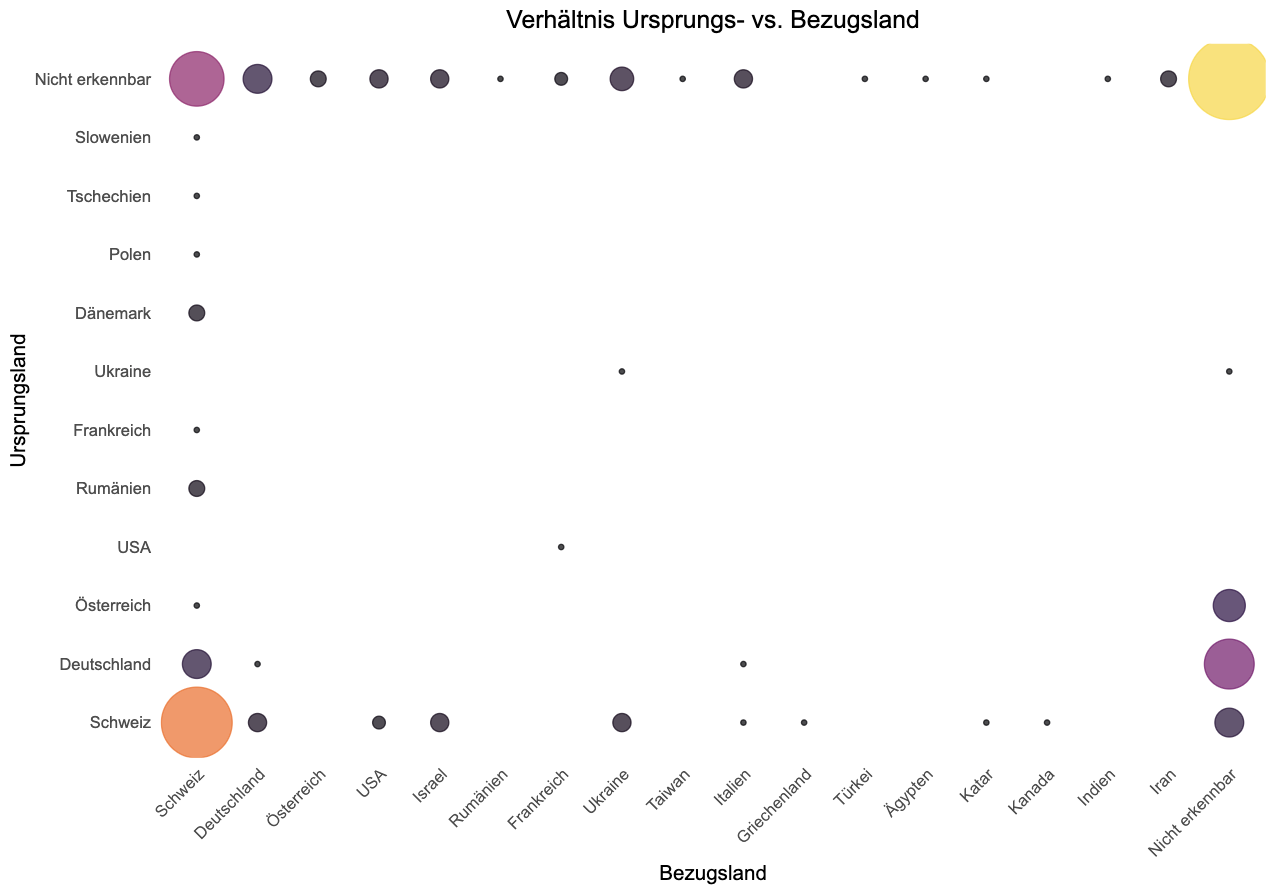
\includegraphics[width=1\linewidth]{images/country_relation_plot.png}
  \footnotesize\textit{Anmerkung.} Eigene Darstellung.
\end{figure}

Erwartungsgemäss thematisierten viele Schweizer Beiträge Themen aus der Schweiz (20,73 \%). Dies dürfte alleine schon gegeben sein aufgrund des Auswahlkriteriums, dass es sich um Beiträge handelt, welche durch die Faktencheck-Plattformen mit Fokus auf die Schweiz ausgewertet wurden. Allerdings ist bei den Beiträgen oft auch kein klares Ursprungs- oder Bezugsland auszumachen (Modus; 27,82 \%). Weiter berichten Schweizer und Schweizerinnen immer wieder über Themen aus dem Ausland, insbesondere über Deutschland, Israel und die Ukraine. Dies passt zum untersuchten Zeitraum, in welchem sich sowohl der Ukrainekrieg als auch der Angriff der Hamas am 7. Oktober 2023 auf Israel ereignete.\\
Ein \(\chi^2\)-Test mit Monte-Carlo-Simulation zeigte keinen statistischen Zusammenhang zwischen Herkunftsland und Bezugsland der Beiträge (10.000 Simulationen; \(\chi^2\) (df = 187, \textit{n} = 381) = 291,7,  \textit{p} = .17).

\textbf{Auditive Videomerkmale}\\
Für jedes Video wurde untersucht, welche audio-spezifische Haupt-Ausprägung das Video hat. Unterschieden wurde zwischen Sprache, Musik und Umgebungsgeräuschen. In Tabelle \ref{tab:results_auditive_specifications} ist die Häufigkeitsverteilung der auditiven Merkmale dargestellt:
\begin{table}[H]
  \caption{\textit{Relative Häufigkeitsverteilung der auditiven Merkmale der Beitrags-Videos in \%}}
  \label{tab:results_auditive_specifications}
  \centering
  \begin{tabular}{|l|l|l|} \hline
    \textbf{Auditives Merkmal} & \textbf{Anzahl Beiträge \textit{n}}& \textbf{Relative Häufigkeit \({h_n}{x_i}\)} \\ \hline
    Sprache & 59 & 81.94 \\ \hline
    Musik & 8 & 11.11 \\ \hline
    Umgebungsgeräusche & 5 & 6.94 \\ \hline
  \end{tabular}
  \footnotesize\textit{Anmerkung.} Eigene Darstellung.
\end{table}
Mit Abstand den grössten Teil der auditiven Ebene von desinformierenden Videos machen Videos mit gesprochenem Text aus (Modus; 81.94 \%).

\subsection{Hypothesen}
\textbf{Thematischer Bezug auf aktuelle Themen}:\\
Als Hypothese 1 wurde angenommen, dass die Verbreitung visueller und audiovisueller Desinformation auf Social-Media-Plattformen in der Schweiz in den letzten Jahren zugenommen hat. Insbesondere während Krisenzeiten (beispielsweise Covid-19-Pandemie, Ukraine-Konflikt, Israel-Konflikt, …) ist ein Anstieg zu erwarten.
Ausgehend vom untersuchten Datensatz ist eine leichte Tendenz erkennbar, dass Desinformation generell über die Jahre zugenommen hat. Dies ist allerdings mit Vorsicht zu geniessen, da dies nur die Anzahl Beiträge widergibt, welche durch die Faktencheck-Plattformen untersucht wurden.\\
Tabelle \ref{tab:results_posts_per_year} zeigt die Anzahl der geposteten Beiträge pro Jahr. Das Jahr 2025 ist ausgenommen, da dieses zum Untersuchungsabschluss noch nicht fertig ist:
\begin{table}[H]
  \caption{\textit{Anzahl untersuchte Beiträge pro Jahr}}
  \label{tab:results_posts_per_year}
  \centering
  \begin{tabular}{|l|l|} \hline
    \textbf{Jahr} (Ausgenommen 2025) & \textbf{Anzahl Beiträge \textit{n}}\\ \hline
    2020& 24\\ \hline
    2021& 126\\ \hline
    2022& 68\\ \hline
    2023&73\\\hline
    2024&80\\\hline
  \end{tabular}\\
  \footnotesize\textit{Anmerkung.} Eigene Darstellung.
\end{table}
\begin{figure}[H]
    \caption{\textit{Liniendiagramm der Beiträge pro Jahr}}
    \label{fig:results_posts_per_year_plot}
    \centering
    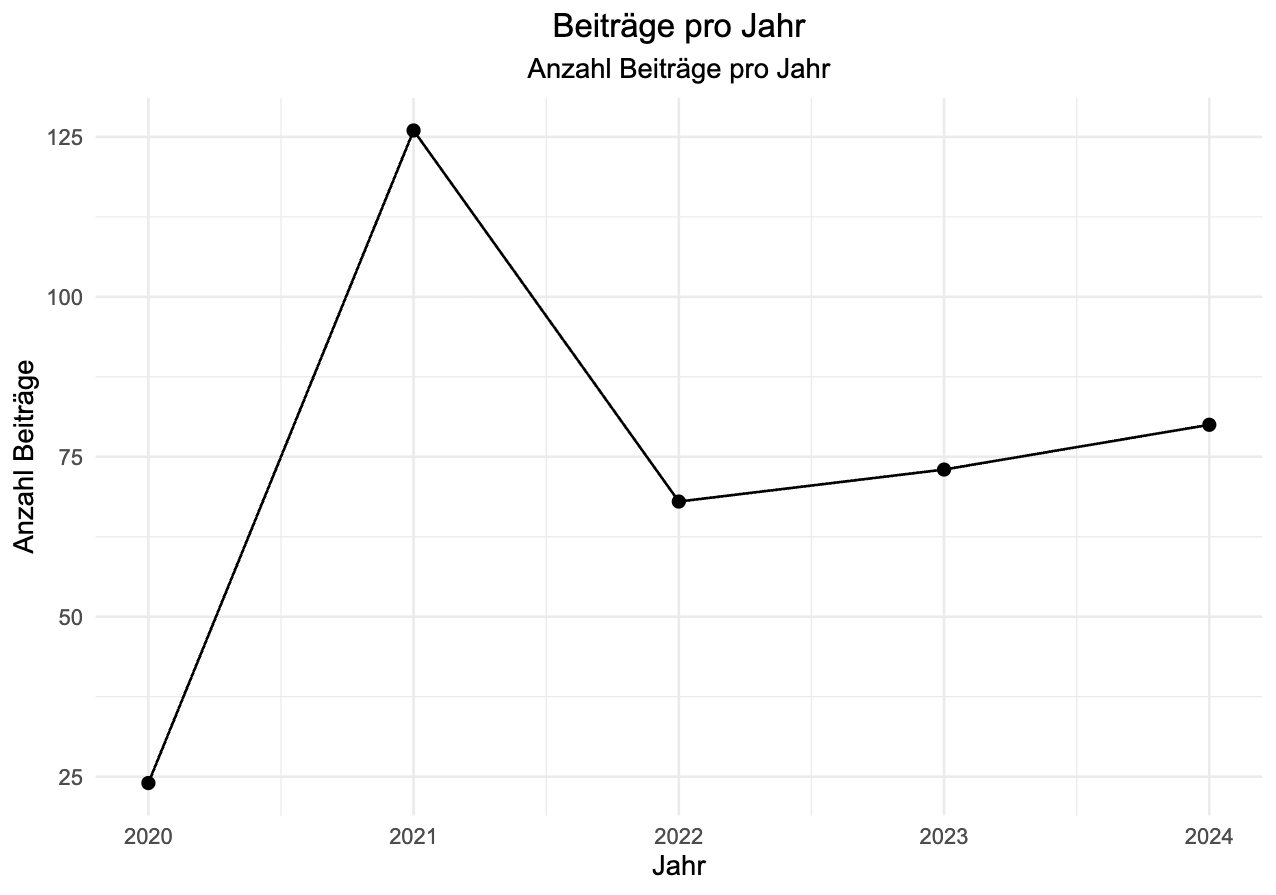
\includegraphics[width=0.75\linewidth]{images/posts_per_year_plot.png} \\
      \footnotesize\textit{Anmerkung.} Eigene Darstellung.
\end{figure}
Diese Häufigkeitsauswertung legt jedoch weiter nahe, dass die Verbreitung von Desinformation themenabhängig ist. Deshalb wurde die Verteilung über die Zeit analysiert. Abbildung \ref{fig:results_date_dependency} zeigt die Anzahl der desinformierenden Beiträge in Abhängigkeit vom Datum und Beitragsthema. Die Grösse der Kreise symbolisiert die Anzahl Beiträge. \\
Bezogen auf die Gesamtzahl aller untersuchten Beiträge (vgl. Tabelle \ref{tab:results_post_topic}  \nameref{tab:results_post_topic}) sind im definierten Zeitraum insbesondere Gesundheit, Politik und Wissenschaft von Bedeutung.
\begin{figure}[H]
  \caption{\textit{Verteilung der Beiträge nach Thema über die Zeit}}
  \label{fig:results_date_dependency}
  \centering
  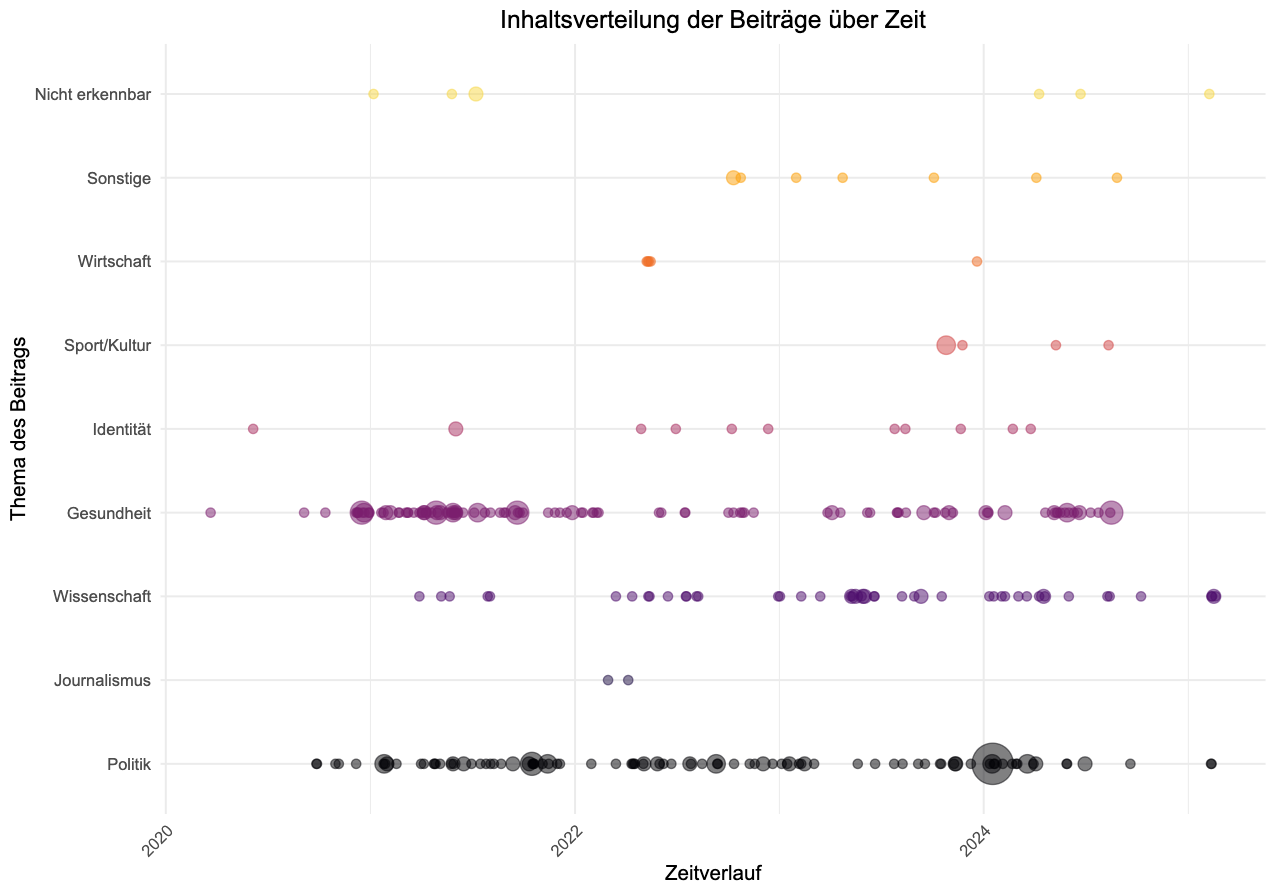
\includegraphics[width=1\linewidth]{images/date_dependency_plot.png}
  \footnotesize\textit{Anmerkung.} Eigene Darstellung.
\end{figure}

Wie zu erwarten war, wird Desinformation zu allen thematischen Kategorien verbreitet. Ausgehend von der Annahme, dass die Verbreitung von Inhalten auf den sozialen Medien der Information des Umfelds dient \parencites[77]{lecheler_disinformation_2022}{subramanian_meet_2017} liess sich, wie in Abbildung \ref{fig:results_date_dependency} dargestellt, zeigen, dass sich die geteilte Desinformation oft auf wichtige aktuelle Themen bezieht.
Über Politik und Gesundheit wurde durchgängig viel berichtet. Andere Themen traten punktuell auf.

\textbf{Emotionalisierung}:\\
Der aktuelle Forschungsstand zu Desinformation lässt als Hypothese 2 vermuten, dass Desinformation bewusst emotionalisierend und provokativ gestaltet wird, da entsprechende Beiträge auf Social Media eine höhere Retention und Interaktion mit sich bringen \parencites[vgl.\ dazu][8]{burkhardt_history_2017}[42]{levak_disinformation_2020}[18]{grujic_warnhinweise_2024}[5]{tandoc_jr_facts_2019}[170]{wahl_fake_2021}. \\
Mit der angewandten Methode war es nahezu unmöglich, zu überprüfen, wie ein Beitrag wahrgenommen wird. Es wurde deshalb untersucht, welche Emotion durch die Posts am wahrscheinlichsten vermittelt werden sollte. Hierfür wurden der Beitragstext und das visuelle Artefakt basierend auf \textcite[1164]{russell_circumplex_1980} nach den folgenden Emotionen kategorisiert: Freude/Humor, Trauer, Wut/Ärger, Anwiderung, Angst und Überraschung/Erstaunen.
Die Häufigkeitsauswertung, dargestellt in Abbildung \ref{fig:results_sentiment_plot}, ergab sowohl für den Beitragstext als auch für das visuelle Artefakt, dass Emotionalität in den Postings eingesetzt wurde.

\begin{figure}[H]
  \caption{\textit{Vergleich der vermittelten Beitrags- und Artefakt-Emotionalität}}
  \label{fig:results_sentiment_plot}
  \centering
  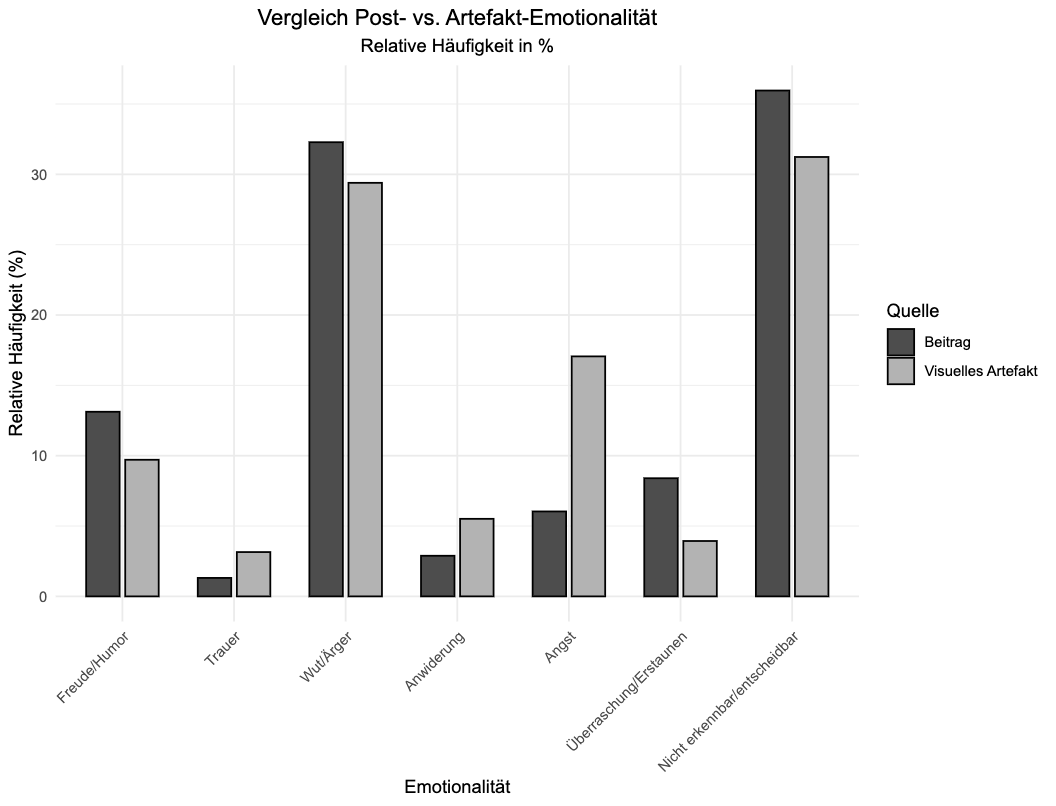
\includegraphics[width=1\linewidth]{images/sentiment_plot.png}
  \footnotesize\textit{Anmerkung.} Eigene Darstellung.
\end{figure}
Abgesehen von den Posts, bei welchen die vermittelte Emotionalität nicht erkennbar war, bildete Wut/Ärger die grösste Kategorie, bei den Beitragstexten als auch bei den visuellen Artefakten (Modus; 32,28 \% / 29,4 \%).

\begin{table}[H]
  \caption{\textit{Kreuztabelle zwischen textlicher und visueller Emotionalität der Beiträge}}
  \label{tab:sentiment_coherence_xtable}
  \centering
  \resizebox{\textwidth}{!}{
    \begin{tabular}{|c|c|c|c|c|c|c|c|} \hline
      \textbf{Beitrags-Emotionalität}& \textbf{Freude/Humor} & \textbf{Trauer} & \textbf{Wut/Ärger} & \textbf{Anwiderung} & \textbf{Angst} & \textbf{Überraschung/Erstaunen} & \textbf{Nicht erkennbar} \\ \hline
      Freude/Humor & 11 & 2 & 12 & 2 & 3 & 2 & 18\\ \hline
      Trauer & 0 & 3 & 1 & 0 & 0 & 0 & 1\\ \hline
      Wut/Ärger & 10 & 4 & 45 & 4 & 14 & 1 & 45\\ \hline
      Anwiderung & 1 & 0 & 3 & 4 & 1 & 0 & 2\\ \hline
      Angst & 0 & 0 & 1 & 0 & 15 & 0 & 7\\ \hline
      Überraschung/Erstaunen & 1 & 0 & 3 & 2 & 5 & 7 & 14\\ \hline
      Nicht erkennbar & 14 & 3 & 47 & 9 & 27 & 5 & 32\\ \hline
    \end{tabular}
  }
  \footnotesize\textit{Anmerkung.} Eigene Darstellung.
\end{table}
Die Untersuchung zeigte, dass insbesondere Wut und Angst, aber auch Freude oder Humor in vielen Beiträgen verwendet wurden. Während die vermittelte Emotionalität bei einigen Beiträgen zwischen Text und Artefakt übereinstimmte, zeigten andere Beiträge keine direkte Überschneidung, beispielsweise, wenn visuelle Darstellungen aus dem Zusammenhang herausgerissen und anders präsentiert wurden. Es fällt ausserdem auf, dass oft humoristische oder sarkastische Beiträge mit Wut im visuellen Artefakt kombiniert wurden.

Um den Zusammenhang zwischen Beitrags-Emotionalität und Emotionalität des visuellen Artefakts statistisch festzustellen und eine Aussage über die Grundgesamtheit treffen zu können,  wurde ein \(\chi^2\)-Test mit Monte-Carlo-Simulation (10.000 Simulationen) durchgeführt. Dieser ergab folgende Werte: \(\chi^2\) (df = 36, \textit{n} = 381) = 178,03, \textit{p} = .00009.\\
Mittels Cramér's V wurde eine Effektstärke von \(\phi_c\) = +0,28 errechnet. Zwischen der vermittelten Emotionalität des Beitrags und des visuellen Begleit-Artefakts besteht somit ein schwacher bis mittlerer Zusammenhang.

\textbf{Spezifische Keywords}: \\
In Fortführung der Filterblasen-Theorie \parencites[vgl.\ bspw.][8]{zoglauer_konstruierte_2021}[222]{schmidt_meinungsbildung_2022}[195]{krafft_disinformation_2020}[8]{grujic_warnhinweise_2024}[221]{allcott_social_2017} werden in Beiträgen möglicherweise spezifische Keywords gesetzt, um so möglichst viel Aufmerksamkeit auf einen Beitrag und so möglichst in diese Blasen einzudringen (Hypothese 3). 
Von den 381 untersuchten Beiträgen beinhalteten 37 (9,71 \%) mindestens ein Keyword/Hashtag. Meist enthielt ein Beitrag mehr als ein Keyword (\textit{n} = 26, 70,27 \%). Grösstenteils stimmten die Keywords mit dem Thema des Beitrags überein (72,97 \%).

Durch Zählung der Beiträge mit Keywords und Gruppierung in Themen wurde die relative Häufigkeit an Beiträgen mit Keyword pro Thema und somit die Wahrscheinlichkeit in \% für jedes Thema errechnet, dass ein zugehöriger Beitrag Keywords enthält (Tabelle \ref{tab:results_tag_likeliness_per_topic}):
\begin{table}[H]
  \caption{\textit{Relative Häufigkeit der Beiträge mit Keyword pro Themengebiet}}
  \label{tab:results_tag_likeliness_per_topic}
  \centering
  \resizebox{\textwidth}{!}{
    \begin{tabular}{|c|c|c|c|} \hline
      \textbf{Thema}&  \textbf{Anzahl Beiträge \textit{n}}&  \textbf{Anzahl Beiträge \textit{n} mit Keywords}& Relative Häufigkeit \({h_n}{x_i}\)\\ \hline
      Politik&  133&  22& 16.54\\ \hline
      Journalismus&  2&  0&  0\\ \hline
      Wissenschaft/Technik&  55&  4&  7.27\\ \hline
      Gesundheit/Medizin&  151&  10&  6.62\\ \hline
      Identität&  12&  0&  0\\ \hline
      Sport/Kultur&  6&  0&  0\\ \hline
      Wirtschaft&  5&  0&  0\\ \hline
      Sonstige& 8& 1&12.5\\\hline
      Nicht erkennbar& 9& 0&0\\\hline
  \end{tabular}}
  \footnotesize\textit{Anmerkung.} Eigene Darstellung.
\end{table}
Politik (Modus; 16,54 \%), Wissenschaft (7,27 \%) und Gesundheit (6,62 \%) waren die einzigen klar definierten Oberthemen, bei denen die Beiträge Keywords enthielten. \\
Unter den sonstigen Beiträgen betrug der Anteil 12,5 \%, allerdings war hier die Anzahl der Beiträge mit Keywords allgemein sehr klein und deshalb nur eine geringe Aussage möglich. 

Aufgrund der Tatsache, dass lediglich 9.71 \% der Beiträge Keywords enthielten, kann nicht davon ausgegangen werden, dass Keywords eine spezielle Rolle spielen bei der Verbreitung von Desinformation. 

\textbf{Distribution}:\\
Basierend auf der These, dass Beiträge auf Social Media vor allem dem Informationsaustausch und dem Ausdruck der eigenen Meinung dienen \parencites[vgl.\ dazu][77]{lecheler_disinformation_2022}{subramanian_meet_2017}[182]{weidner_fake_2019}, wird mit Hypothese 4 angenommen, dass auch desinformierende Beiträge primär von Privatpersonen mit unterschiedlichen gesellschaftlichen Rollen geteilt werden.

Für die Auswertung wurde für jeden Beitrag erhoben, ob es sich um einen Individual- oder Kollektivakteur handelt, und welcher gesellschaftlichen Rolle der Account zugeordnet werden kann. Anschliessend wurde jeweils die relative Häufigkeit \({h_n}{x_i}\) in Relation zum Akteurstyp ausgewertet.

\begin{figure}[H]
  \caption{\textit{Relative Häufigkeit der Akteursrollen innerhalb der Akteurstypen}}
  \label{fig:results_actor_plot}
  \centering
  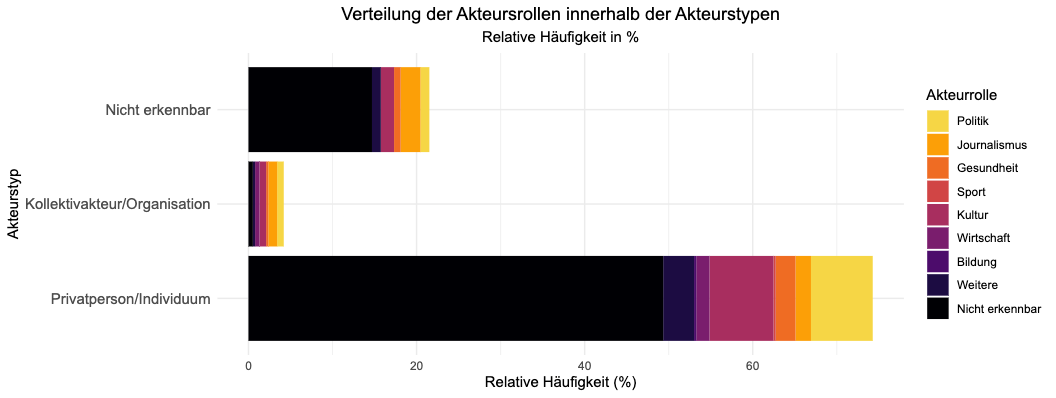
\includegraphics[width=1\linewidth]{images/actor_plot.png}
  \footnotesize\textit{Anmerkung.} Eigene Darstellung.
\end{figure}
Die Häufigkeitsverteilung der Akteurstypen ergab, dass es sich in etwa drei Viertel (Modus; 74,28 \%) der Fälle um Privatpersonen handelte, welche die Desinformation auf Social Media teilten. Bei 4,21 \% handelte es sich um Kollektivakteure, der Rest war nicht klar erkennbar.\\
Abbildung \ref{fig:results_actor_plot} zeigt die Verteilung der Akteursrollen im Gesamtverhältnis zur relativen Häufigkeit der Akteurstypen.

Innerhalb der Akteurstypen waren die gesellschaftlichen Rollen unterschiedlich verteilt, dargestellt in Tabelle \ref{tab:results_actor_xtable} \nameref{tab:results_actor_xtable}.\\
Neben Privatpersonen ohne erkennbare gesellschaftliche Rolle waren bei den Privatpersonen Kultur (Modus; 7.61 \%) und Politik (7.35 \%) besonders stark ausgeprägt, bei den Kollektivakteuren waren journalistische Akteure (4.21 \%) am stärksten vertreten. Insgesamt herrschte bei den Kollektivakteuren eine gleichmässigere Verteilung der Akteurrolle.
\begin{table}[H]
    \centering
\caption{Kreuztabelle zwischen Akteurstyp und gesellschaftlicher Rolle}
\label{tab:results_actor_xtable}
      \resizebox{\textwidth}{!}{
    \begin{tabular}{|c|c|c|c|c|c|c|c|c|c|}\hline
         \textbf{Akteurstyp}&  Politik&  Journalismus&  Gesundheit&  Identität&  Sport/Kultur&  Wirtschaft&  Bildung&  Weitere& Nicht erkennbar\\\hline
         Individualakteur&  28&  7&  9&  1&  29&  6&  1&  14& 188\\\hline
         Kollektivakteur&  3&  4&  1&  0&  3&  2&  0&  1& 2\\\hline
         Nicht erkennbar&  4&  9&  3&  0&  6&  0&  0&  4& 56\\ \hline
    \end{tabular}
    }
    \footnotesize\textit{Anmerkung.} Eigene Darstellung.
\end{table}

Der \(\chi^2\)-Test mit Monte-Carlo-Simulation (10.000 Simulationen) ergab einen Zusammenhang zwischen Akteurstyp und seiner gesellschaftlichen Rolle: \(\chi^2\) (df = 18, \textit{n} = 381) = 44,6, \textit{p} = .0081, mit einer Effektstärke von \(\phi_c\) = +0.24. 

Um herauszufinden, inwiefern die Rolle eines Akteurs mit dem Thema des Beitrags in Zusammenhang steht, wurde auch für die Kreuztabelle zwischen Beitragsthema und Akteursrolle (s. Tabelle \ref{tab:results_role_topic_xtable} \nameref{tab:results_role_topic_xtable}) ein \(\chi^2\)-Test mit Monte-Carlo-Simulation (10.000 Simulationen) berechnet:  \(\chi^2\) (df = 64, \textit{n} = 381) = 52,54, \textit{p} = .57. Die Effektstärke betrug gemäss Cramér's V \(\phi_c\) = +0.13. Der \(\chi^2\)-Test ergab keinen statistischen Zusammenhang zwischen gesellschaftlicher Rolle und Beitragsthema, das Beitragsthema eines geposteten Beitrags ist statistisch unabhängig von der gesellschaftlichen Rolle des verbreitenden Akteurs.

\begin{table}
    \centering
\caption{\textit{Kreuztabelle zwischen Akteurrolle und Beitragsthema}}
\label{tab:results_role_topic_xtable}
     \resizebox{\textwidth}{!}{
    \begin{tabular}{|c|c|c|c|c|c|c|c|c|l|}\hline
         \textbf{Akteurrolle}&  \textbf{Politik}&  \textbf{Journalismus}&  \textbf{Wissenschaft}&  \textbf{Gesundheit}&  \textbf{Identität}&  \textbf{Sport/Kultur}&  \textbf{Wirtschaft}& \textbf{Sonstige} &\textbf{Nicht erkennbar}\\\hline
         Personen der Politik&  16&  0&  7&  8&  3&  1&  0&  0&0\\\hline
         Journalismus&  3&  0&  4&  12&  0&  0&  0&  0&1\\\hline
         Gesundheitswesen&  1&  0&  1&  9&  1&  0&  0&  1&0\\\hline
         Identität&  0&  0&  0&  1&  0&  0&  0&  0&0\\\hline
         Kultur&  20&  0&  3&  13&  0&  1&  0&  0&1\\\hline
         Wirtschaft&  3&  0&  3&  2&  0&  0&  0&  0&0\\\hline
         Bildungswesen&  1&  0&  0&  0&  0&  0&  0&  0&0\\\hline
         Weitere&  6&  0&  2&  8&  0&  0&  0&  2&1\\ \hline
         Nicht erkennbar&  83&  2&  35&  98&  8&  4&  5&  5&6\\ \hline
    \end{tabular}
    }\\
    \footnotesize\textit{Anmerkung.} Eigene Darstellung.
\end{table}
Erwartungsgemäss berichteten Akteure oft über ihr eigenes Fachgebiet oder innerhalb ihres eigenen Themenumfelds. Akteure aus dem journalistischen Bereich und der Politik berichteten über diverse Themen. Ebenso taten dies Akteure aus dem Kulturumfeld, beispielsweise Influencerinnen und Influencer.\\

\textbf{Technische Komplexität}:\\
Für Hypothese 5 wird ausgehend von \textcite [15]{bradshaw_industrialized_2021} und \textcite[3698]{weikmann_visual_2023} davon ausgegangen, dass es sich bei den visuellen Artefakten um Artefakte mit tiefer technischer Komplexität handelt, da diese weniger aufwendig sind in der Produktion.

Die Komplexität der visuellen Artefakte wurde über eine Häufigkeitsverteilung erfasst. Hierfür wurden statische Grafiken unterteilt in "ohne Bearbeitung", "tiefe Komplexität", "hohe Komplexität", irreführende Datenvisualisierung und eigens erstellte Grafiken, beispielsweise Memes oder Bildcollagen. Videos wurden unterschieden in "ohne Bearbeitung", "tiefe Komplexität" (Filter, Geschwindigkeitsänderungen), "mittlere Komplexität" (Veränderung der Bildkomposition oder Einfügen von Grafiken, Animationen, \ldots) und "hohe Komplexität" (Deep Fakes, Virtual Performances).
\begin{figure}[H]
  \caption{\textit{Häufigkeitsverteilung der Artefakt-Typen}}
  \label{fig:results_artefact_type}
  \centering
  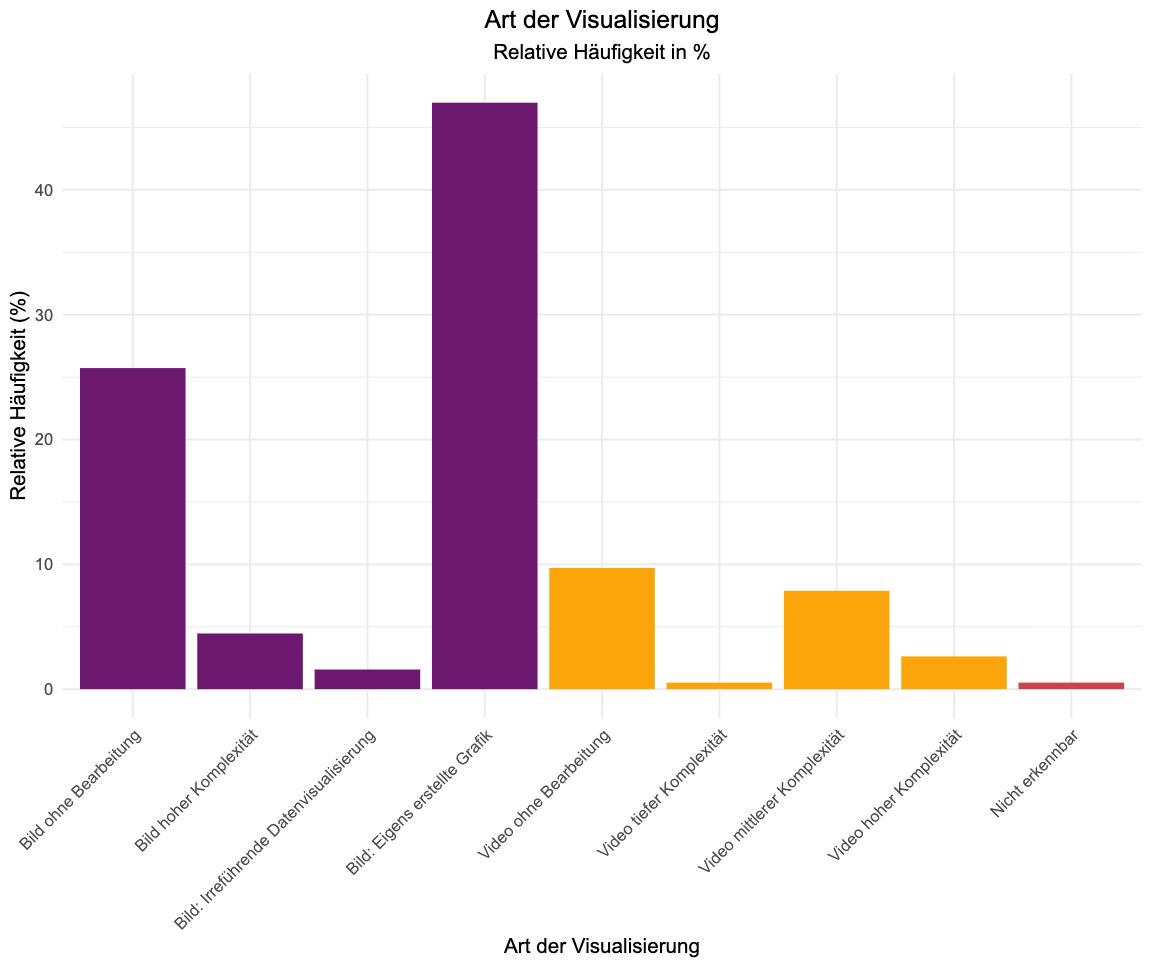
\includegraphics[width=0.75\linewidth]{artefact_type_plot.png}\\
  \footnotesize\textit{Anmerkung.} Eigene Darstellung.
\end{figure}
Den anteilsmässig grössten Teil der visuellen Artefakte machten, wie in Abbildung \ref{fig:results_artefact_type} erkennbar, eigens erstellte Grafiken aus (Modus; 46,98 \%). Darunter zählen beispielsweise Memes, rein textbasierte Bilder oder Fotos mit Begleittext im visuellen Artefakt. \\
Einen weiteren grossen Anteil hatten reine Bilder, bei welchen keine Bearbeitung erkennbar war (25,72 \%). Insgesamt handelte es sich bei desinformierenden Bildern meist um Darstellungen, welche aus dem Kontext gerissen dargestellt wurden. Bildmanipulationen (Bild hoher Komplexität, 4,46 \%) konnten selten festgestellt werden.

Videos machten rund einen Fünftel der visuellen Artefakte aus (20,47 \%). Den grössten Anteil hatten Videos ohne Bearbeitung (9,71 \% aller Artefakte), Videos mittlerer Komplexität (einfache Schnitte, Grafikeinblendungen und Animationen) machten 7,87 \% aller Artefakte aus. Videos mit hoher technischer Komplexität wurden selten gepostet (2,62 \%).

\textbf{Inhaltlicher Zusammenhang}:\\
\Textcite[15]{bradshaw_industrialized_2021} und \textcite[3700]{weikmann_visual_2023} verweisen darauf, dass bei Desinformation auf Social Media oftmals wahre Ereignisse und Gegebenheiten falsch wiedergegeben werden.
Davon ausgehend wird als Hypothese 6 angenommen, dass die effektive Desinformation in der Regel im Begleittext des Beitrags verortet ist und das mediale Artefakt diese Aussage des Begleittextes stützt. \\

Zur Analyse des inhaltlichen Zusammenhangs zwischen dem Beitrag und dem visuellen Artefakt wurde eine Häufigkeitsauswertung vorgenommen. Die Ergebnisse sind in Tabelle \ref{tab:results_visual_coherence_table} ersichtlich.

\begin{table}[H]
  \caption{\textit{Häufigkeitsauswertung des inhaltlichen Zusammenhangs zwischen Beitragstext und visuellem Artefakt}}
  \label{tab:results_visual_coherence_table}
  \centering
  \begin{tabular}{|l|l|l|}\hline
    \textbf{Inhaltliche Kohärenz}&  \textbf{Anzahl Beiträge \textit{n}}& \textbf{Relative Häufigkeit \({h_n}{x_i}\)}\\\hline
    Text sachlich, Artefakt sachlich&  7& 1.84\\\hline
    Text sachlich, Artefakt desinformierend&  8& 2.1\\\hline
    Text desinformierend, Artefakt sachlich&  93& 24.41\\\hline
    Text und Artefakt desinformierend&  176& 46.19\\\hline
    Nicht erkennbar&  97& 25.46\\ \hline
  \end{tabular}
  \footnotesize\textit{Anmerkung.} Eigene Darstellung.
\end{table}
In 46,19 \% (Modus) der Fälle waren sowohl der Beitragstext als auch das begleitende Bild oder Video desinformierend. Einen weiteren grossen Anteil machten Beiträge aus, bei welchen lediglich der Beitragstext desinformierend war (24,41 \%), beispielsweise indem Bilder, Grafiken oder Videos aus dem Zusammenhang herausgerissen und falsch dargestellt wurden. Bei etwa einem Viertel (25,46 \%) war der inhaltliche Zusammenhang nicht erkennbar, beispielsweise, weil kein Beitragstext vorhanden war und nur das visuelle Artefakt geteilt wurde.\\
 Es kann also davon ausgegangen werden, dass desinformierende Beiträge in einem Grossteil der Fälle entweder komplett falsch sind oder zumindest falsch über ein wahres visuelles Artefakt berichtet wird.

Weiter wurde untersucht, in welchem Zusammenhang das Thema des Beitrags mit dem Thema des visuellen Begleitartefakts steht. Hierfür wurden die einzelnen Codierungen für die Thematik der visuellen Artefakte thematisch zusammengefasst und eine Häufigkeitsauswertung des Artefakt-Themas in Relation zum Beitragsthema vorgenommen.
\begin{figure}
  \caption{\textit{Thematisches Verhältnis zwischen dem Thema des Beitrags und des visuellen Artefakts}}
  \label{fig:results_visual_coherence_plot}
  \centering
  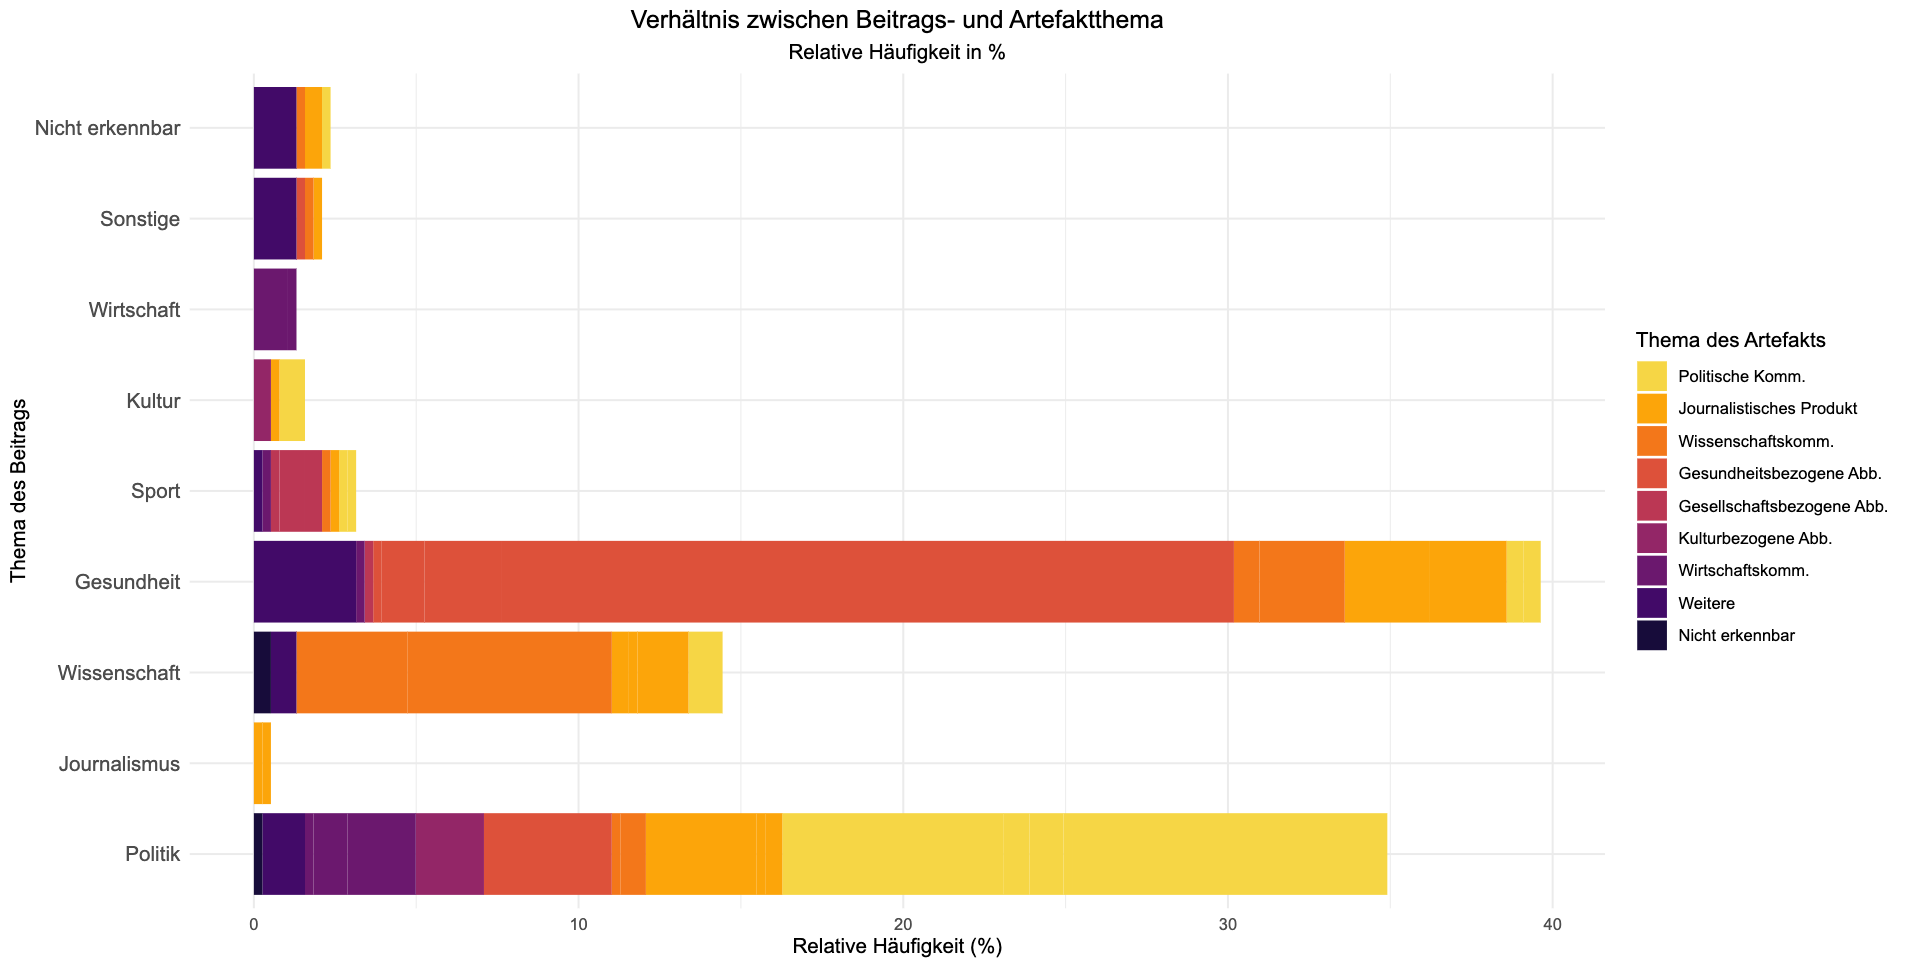
\includegraphics[width=1\linewidth]{images/visual_coherence_plot.png}
  \footnotesize\textit{Anmerkung.} Eigene Darstellung.
\end{figure}
Wie in Abbildung \ref{fig:results_visual_coherence_plot} erkennbar ist, fiel in vielen Fällen das Beitragsthema mit dem Thema des visuellen Artefakts zusammen. Besonders stark war diese thematische Überschneidung bei den Themen Gesundheit, Wissenschaft, Journalismus und Politik.

Um den Zusammenhang zwischen Beitrags- und Artefakt-Thema statistisch festzustellen, wurde eine Kreuztabelle zwischen den beiden Variablen erstellt (Tabelle \ref{tab:results_visual_coherence_xtable} \nameref{tab:results_visual_coherence_xtable}):

\begin{table}[H]
    \caption{\textit{Kreuztabelle zwischen Thematik des Beitrags und des visuellen Artefakts}}
    \label{tab:results_visual_coherence_xtable}
    \centering
     \resizebox{\textwidth}{!}{
    \begin{tabular}{|c|c|c|c|c|c|c|c|c|c|}\hline
         \textbf{Beitragsthema}&  Politische Kommunikation&  Journalistisches Produkt&  Wissenschaftskommunikation&  Gesundheitsbezogene Abbildung&  Gesellschaftsbezogene Abbildung&  Kulturbezogene Abbildung&  Wirtschaftskommunikation&  Weitere& Nicht erkennbar\\\hline
         Politik&  71&  16&  4&  15&  0&  0&  0&  5& 1\\\hline
         Journalismus&  0&  2&  0&  0&  0&  0&  0&  0& 0\\\hline
         Wissenschaft&  4&  9&  37&  0&  0&  0&  0&  3& 2\\\hline
         Gesundheit&  4&  19&  13&  101&  1&  0&  1&  12& 0\\\hline
         Identität&  2&  1&  1&  0&  6&  0&  1&  1& 0\\\hline
         Sport/Kultur&  3&  1&  0&  0&  0&  2&  0&  0& 0\\\hline
         Wirtschaft&  0&  0&  0&  0&  0&  0&  5&  0& 0\\\hline
         Sonstige&  0&  1&  1&  1&  0&  0&  0&  5& 0\\\hline
         Nicht erkennbar&  1&  2&  1&  0&  0&  0&  0&  5& 0\\ \hline
    \end{tabular}
}
\footnotesize\textit{Anmerkung}. Eigene Darstellung.
\end{table}
Die Berechnung von \(\chi^2\) mit Monte-Carlo-Simulation (10.000 Simulationen) ergab folgende Werte: \(\chi^2\) (df = 64, \textit{n} = 381) = 694.75, \textit{p} = .00009999. Die Effektstärke betrug \(\phi_c\) = 0,48,  was auf einen mittelstarken Bezug zwischen den beiden Variablen hindeutet.

\textbf{Erstellungszweck}:\\
Bei Hypothese 7 wird davon ausgegangen, dass Desinformation jeweils aus einem bestimmten Grund verbreitet wird. Für diese Auswertung wurden die Beiträge inhaltlich analysiert und entsprechend kategorisiert.

Pro Beitrag wurde aufgrund der definierten Kategorien der inhaltliche Erstellungszweck als Häufigkeitsverteilung ausgewertet. Die Ergebnisse sind in Tabelle \ref{tab:results_content_creation_purpose} festgehalten.

\begin{table}
  \centering
  \caption{\textit{Häufigkeitsverteilung des inhaltlichen Erstellungszwecks der Beiträge}}
  \label{tab:results_content_creation_purpose}
  \begin{tabular}{|c|c|c|}\hline
    \textbf{Inhaltlicher Erstellungszweck}&  \textbf{Anzahl Beiträge \textit{n}}& Relative Häufigkeit \({h_n}{x_i}\)\\\hline
    Teilen von Informationen&  16& 4.21\\\hline
    Augenzeugenbericht&  5& 1.31\\\hline
    Intimitätsaustausch&  12& 3.15\\\hline
    Persönlicher Standpunkt&  244& 64.04\\\hline
    Unterhaltungszweck&  10& 2.62\\\hline
    Nicht erkennbar&  94& 24.67\\ \hline
  \end{tabular}
  \footnotesize\textit{Anmerkung.} Eigene Darstellung.
\end{table}
Den häufigsten Erstellungszweck bildet der persönliche Standpunkt (Modus; 64,04 \%). Personen verfassen primär Beiträge mit ihrer eigenen Meinung zu einem Thema. Weiter dienten die Beiträge oft dem Teilen von Informationen (4,21 \%) sowie dem Intimitätsaustausch (3,15 \%), wenn über persönliche Erlebnisse berichtet wurde. In rund einem Viertel der Fälle  (24,67 \%) war kein klarer Verbreitungsgrund erkennbar.

\textbf{Video-Schnittgeschwindigkeit}:\\
Hypothese 8 geht davon aus, dass desinformierende Videos zugunsten der höheren Aufmerksamkeitsgenerierung eine hohe Schnitt-Kadenz enthalten.
Zur Evaluation der Schnittgeschwindigkeit wurde die Anzahl der Schnitte der Videos pro Minute für die entsprechenden Beiträge folgendermassen berechnet:
\[CPM  = \frac{\# \ Schnitte}{\frac{Videolänge\ in\ s}{60}}\]
Um eine Referenzlänge für eine normale Schnitt-Kadenz zu erhalten, wurden zusätzlich je drei Social-Media-Videos von SRF, 20 Minuten und Nau.ch auf die gleiche Art ausgewertet.
Abbildung \ref{fig:video_cut_plot} zeigt die absolute Anzahl an Videos, welche eine bestimmte Anzahl Schnitte beinhalteten.

\begin{figure}[H]
  \caption{\textit{Schnittgeschwindigkeit der Video-Artefakte}}
  \label{fig:video_cut_plot}
  \centering
  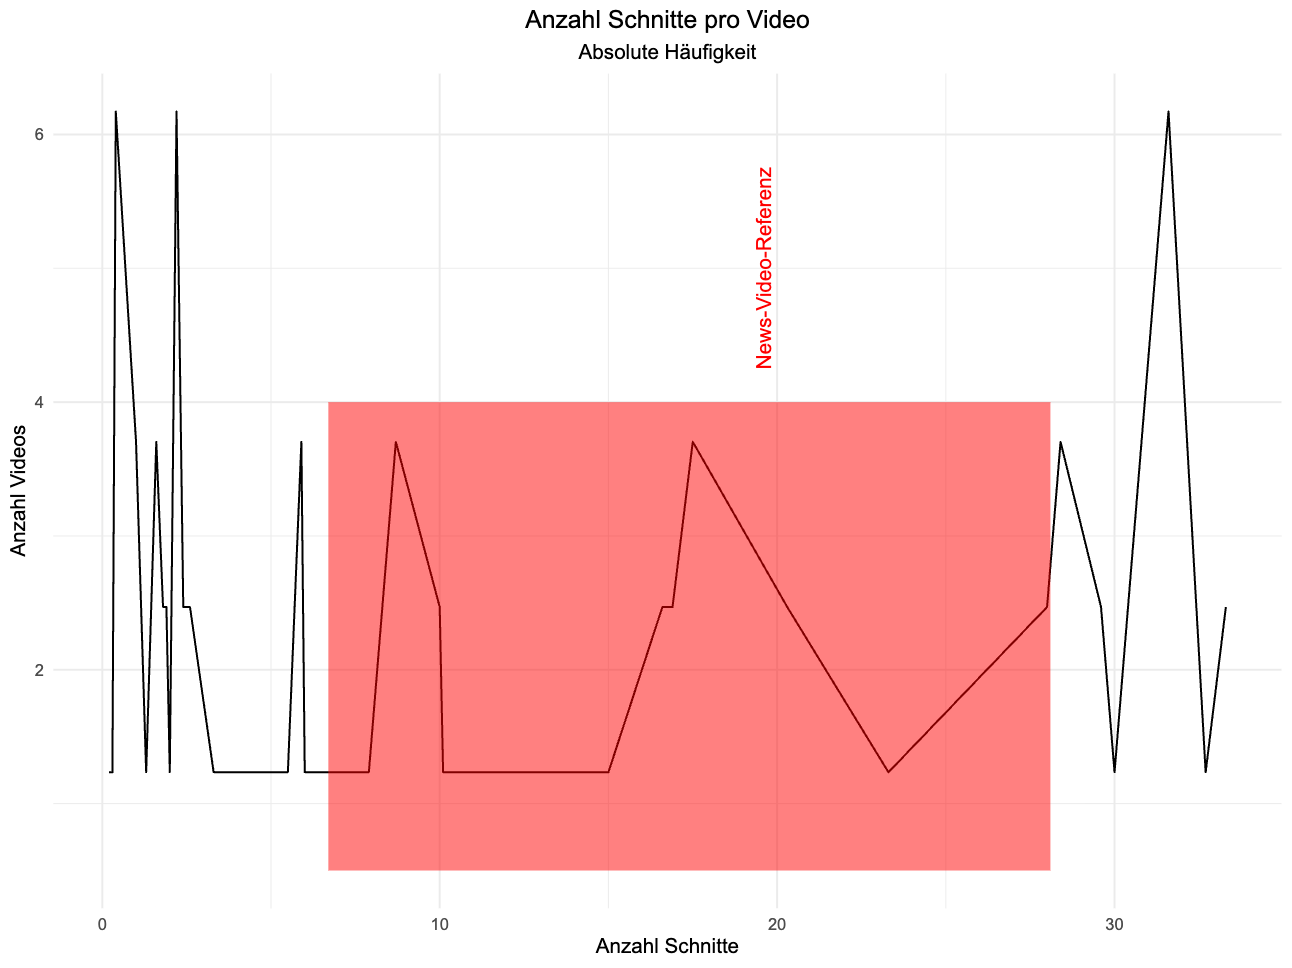
\includegraphics[width=1\linewidth]{images/video_cpm_plot.png}
  \footnotesize\textit{Anmerkung.} Eigene Darstellung.
\end{figure}
Insgesamt konnten von allen Beiträgen 78 Videos ausgewertet werden. Gemäss Hypothese 8 wäre zu erwarten, dass die desinformierenden Videos in der Tendenz rechts des Referenz-Bereichs liegen. 11,54 \% (\textit{n} = 9) der Videos enthielten 1 oder weniger Schnitte pro Minute. 17,95 \% (\textit{n} = 11) liegen über dem Referenzbereich von 1,6-28 Schnitten pro Minute.\\
Hypothese 8 kann somit nicht generell positiv beantwortet werden.

\pagebreak
\section{Forschungsergebnisse}
\subsection{Diskussion}
Diese Arbeit untersucht, wie visuelle und audiovisuelle Desinformation auf Social Media in der Schweiz produziert und verbreitet wird. Hierfür wurde eine quantitative Inhaltsanalyse von desinformierenden Social-Media-Beiträgen durchgeführt und die Resultate im \nameref{sec:results}steil analysiert.

\textbf{Themen}\\
Ausgehend von den untersuchten Beiträgen lässt sich über die letzten Jahre ein leichter Anstieg der Desinformationsbeiträge verzeichnen. Dies ist aufgrund der verwendeten Methode zwar stark von den Faktencheck-Plattformen und der durch sie untersuchten Beiträge abhängig, deckt sich jedoch mit der weiteren Beobachtung, dass sich Desinformation oft auf aktuell wichtige Themen bezieht. Der Anstieg bestätigt die Erkenntnisse unter anderem von \textcite{khan_fake_2021} und \textcite[26]{vogler_wahrnehmung_2021}. 

Thematisch wird Desinformation zu allen untersuchten Themengebieten geteilt, die Beiträge konzentrieren sich jedoch zu einem grossen Teil auf Gesundheit, Politik und wissenschaftliche Themen \parencite[vgl.\ dazu ][2]{ceron_fake_2021}.\\
Die Beiträge dienen dabei in den meisten Fällen dem persönlichen Meinungsaustausch oder dem Mitteilen von Informationen an das Umfeld der Nutzenden.

\textbf{Produktion}\\
Desinformierende Beiträge werden, wie erwartet, oftmals emotionalisiert dargestellt \parencites[vgl.\ dazu][3703]{weikmann_visual_2023}[146]{teixeira_emotion-induced_2012}[23]{zhou_effects_2005}. Insbesondere Wut, Angst und Freude werden oft vermittelt. In vielen Fällen korrespondiert die im Beitrag vermittelte Emotion mit der Emotion des visuellen Artefakts.\\
\textcite[Pennycook et al. (2018), zit\ nach][182]{weidner_fake_2019}, \textcite[15]{bradshaw_industrialized_2021} und \textcite[3700]{weikmann_visual_2023} bestätigend, dass eine gewisse Glaubwürdigkeit vorhanden sein muss, passen die Beitragstexte in der Regel thematisch mit dem visuellen Artefakt zusammen. Oftmals sind entweder beide Komponenten falsch, oder ein Beitrag berichtet desinformierend über ein wahres Bild oder Video.\\
In den untersuchten Beiträgen wurden, unerwartet, eher selten Keywords verwendet, um die Desinformation in einer bestimmten Gruppe zu verbreiten. Keywords scheinen für die Verbreitung der Desinformation aufgrund der vorliegenden Daten eine untergeordnete Rolle zu spielen.

Bei einem grossen Anteil der Beiträge handelt es sich bei den visuellen Artefakten um Bilder. Entgegen der Annahme, dass dabei vor allem einfache Bearbeitungen wie Zuschneiden des Ausschnitts angewendet werden, zeigte sich, dass es sich meistens um echte Bilder handelt oder um Grafiken, bei welchen Text hinzugefügt oder welche bearbeitet wurden.\\ 
Wenn Videos verwendet werden, weisen diese oft keine Bearbeitung auf oder sind nur marginal verändert, beispielsweise durch Schnitte oder das Einfügen von Grafiken. Videos enthalten meist gesprochenen Text. Die Aufmerksamkeitsgenerierung erfolgt nicht spezifisch erkennbar über eine besondere Schnittgeschwindigkeit.

\textbf{Verbreitung}\\
In der Schweiz wird Desinformation vor allem via Facebook, Telegram und X/Twitter geteilt. Dies deckt sich nicht mit den meistgenutzten Social-Media-Plattformen \parencite[vgl.]{we_are_social_fuhrende_2025}. 
Oftmals berichten Schweizerinnen und Schweizer über Themen mit Schweizbezug. Allerdings finden sich auch Beiträge mit Schweizbezug aus anderen Staaten oder Schweizer Beiträge mit einem anderen Bezugsland.

Desinformierende Beiträge werden in der Regel von Privatpersonen verteilt, oftmals ist keine spezifische gesellschaftliche Rolle erkennbar. \\
Obwohl insgesamt kein statistischer Zusammenhang zwischen gesellschaftlicher Rolle und dem Beitragsthema besteht, zeigte sich in der Häufigkeitsauswertung, dass bei der Verbreitung oftmals über Themen des eigenen Themenumfelds berichtet wird. Dieser scheinbare Widerspruch lässt sich möglicherweise auf eine zu kleine Stichprobe für die entsprechende Auswertung zurückführen oder auf die Tatsache, dass bei verhältnismässig vielen Beiträgen keine klare gesellschaftliche Rolle der Verbreitungsakteure erkennbar war.

\subsection{Weiterer Forschungsbedarf}
Die vorliegende Forschung liefert einen Überblick über die Produktions- und Verbreitungsarten der auf Social-Media-Plattformen in der Schweiz verbreiteten Desinformationen. Dabei bildet der Zusammenhang zwischen der textlichen Ebene und den visuellen und audiovisuellen Begleitartefakten den Schwerpunkt der Untersuchung.

Für die Erforschung der Rezeption der Inhalte müssen weitere Untersuchungen durchgeführt werden. Auch über das tatsächliche Ausmass von Desinformation auf Social Media kann keine Aussage getroffen werden.

Für weiterführende Untersuchungen empfiehlt es sich, einen grösseren Datensatz zu untersuchen und gegebenenfalls eine eigene Definitionsgrundlage für die Erfassung von desinformierenden Beiträgen zu entwickeln. Dadurch kann auf die Abhängigkeit von Faktencheck-Plattformen zur Einordnung verzichtet werden, was zu einem akkurateren Gesamtbild der Grundgesamtheit führen könnte. 
\pagebreak
\section{Fazit}
Diese Bachelorarbeit untersuchte, welche Merkmale audiovisuelle und visuelle Desinformation auf Social-Media-Plattformen in der Schweiz aufweist. Hierfür wurde eine quantitative Inhaltsanalyse von Social-Media-Beiträgen durchgeführt, welche von Faktencheck-Plattformen mit Schweizbezug als Desinformation deklariert wurden. Das standardisierte Vorgehen gewährleistet ähnliche Ergebnisse bei wiederholten Untersuchungen oder Auswertungen zu einem späteren Zeitpunkt.\\
Aufgrund dieser Erkenntnisse können Handlungsempfehlungen zur Stärkung der Medienkompetenz und zum Umgang mit visueller und audiovisueller Desinformation auf Social Media abgeleitet werden.

Durch die sozialen Medien, welche heute zumindest eine zentrale Rolle in der persönlichen Information der Bevölkerung spielen, werden Individualpersonen, oft ohne ihr Wissen, journalistisch tätig. Durch falsche und desinformierende Beiträge wird die Wahrnehmung der Rezipierenden massgeblich verzerrt, was dramatische Auswirkungen auf die eigene Meinungsbildung und somit auf demokratische Prozesse haben kann. Dies trifft insbesondere auf direkte Demokratien zu, wie sie die Schweiz hat.

Audiovisuelle Desinformation kann aufgrund der höheren Aufmerksamkeitsgenerierung besonders problematisch sein. Dies wird dadurch verstärkt, dass Rezipierende sich meist besser an visuelle und audiovisuelle Inhalte erinnern als an Text. Inhalten in Video- und Bildform wird zudem meist eine höhere Glaubwürdigkeit zugesprochen. Sie wirken emotionaler und haben einen grösseren Effekt auf die Meinungsbildung der Rezipierenden.

Die Ergebnisse der Inhaltsanalyse belegen, dass Desinformation auf diversen Plattformen und zu allen Themen verbreitet wird, sich aber vor allem auf aktuelle Ereignisse bezieht. Beiträge werden oft emotionalisierend gestaltet, wobei in der Regel der Beitragstext und das visuelle Artefakt sowohl thematisch als auch emotional einen stimmigen Gesamtkontext vermitteln. Zu einem Grossteil werden Bilder oder Grafiken mit einem desinformierenden Begleittext veröffentlicht.\\
Zumeist handelt es sich bei den Akteuren, welche die Desinformation verbreiten, um Einzelpersonen. Meist vermitteln der Beitrag und das visuelle Artefakt einen stimmigen – wenn auch faktisch falschen – Kontext und können so nur schwer als Desinformation identifiziert werden.\\
Diese Ergebnisse bestätigen den bisherigen Forschungsstand sowie die meisten davon abgeleiteten Hypothesen.

Insgesamt gibt es bisher, insbesondere mit Fokus auf die Schweiz, wenig Untersuchungen zu Desinformation auf Social Media. Neben der hier untersuchten Produktions- und Verbreitungsebene von Desinformation dürfte insbesondere ein zusätzlicher Fokus auf die verbreitenden Akteure sowie auf die Rezipierenden von Bedeutung sein. Auch das Ausmass von Desinformation auf Social Media im Vergleich zu allen anderen Beiträgen ist weiterhin unbekannt.

\pagebreak
%-----------------------------------------------
%BIB
\section{Verzeichnisse}
\subsection{Literatur}
\printbibliography[heading=none, nottype=artwork]
\subsection{Bildverweise}
\listoffigures
\listoftables
\subsection{Hilfsmittelverzeichnis}
\pagebreak
\section{Anhang}
\subsection{Codebuch}
~\label{appendix_codebook}
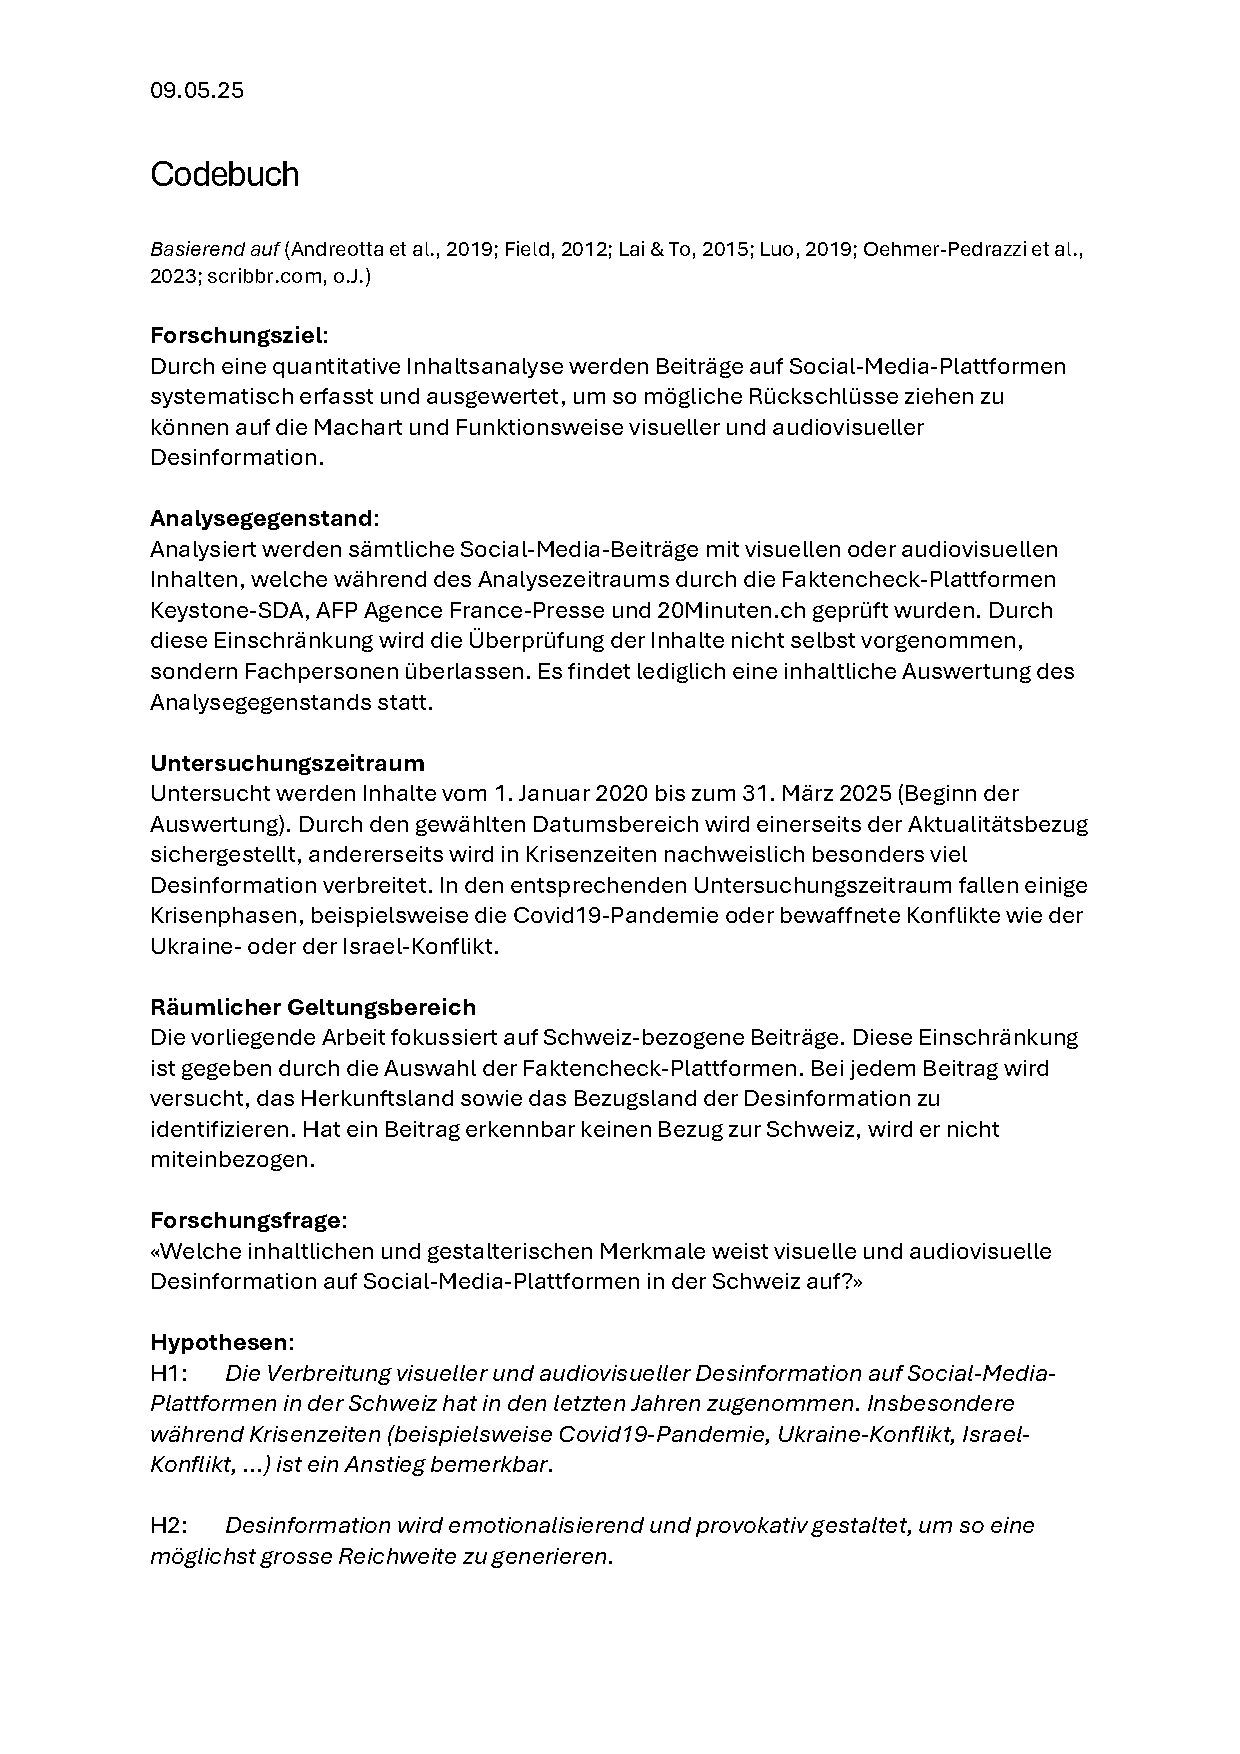
\includepdf[pages={1-14}]{Codebuch-appendix}
\subsection{Python Webcrawler}
~\label{appendix_crawler}
\begin{lstinputlisting}[language=Python, caption=Python Webcrawler für Keystone-SDA]{bsc_crawl_keystone-sda-listing.py}
\end{lstinputlisting}
\begin{tcolorbox}[
    width=\textwidth,    % gesamte Textbreite
    boxrule=1pt,         % Stärke des Rahmens
    arc=0pt,             % quadratische Ecken
    colback=white,       % Hintergrundfarbe
    left=6pt, right=6pt, top=6pt, bottom=6pt
  ]
  \textbf{GitHub}:\\
  \url{https://github.com/y-neck/bsc-thesis/blob/c11abd9801091f22f37d34ecabb817b458cc9171/thesis/bsc_crawl_keystone-sda-listing.py}
\end{tcolorbox}
\subsection{Datensatz}
\label{appendix_dataset}
\begin{tcolorbox}[
    width=\textwidth,    % gesamte Textbreite
    boxrule=1pt,         % Stärke des Rahmens
    arc=0pt,             % quadratische Ecken
    colback=white,       % Hintergrundfarbe
    left=6pt, right=6pt, top=6pt, bottom=6pt
  ]
  \textbf{Der untersuchte Datensatz kann hier heruntergeladen werden}: \\
  \url{https://github.com/y-neck/bsc-thesis/blob/347b14f7573e65201ccfa2710e31633e2a3966fa/dataset.json}
\end{tcolorbox}
\subsection{R Datenanalyse}
\label{appendix_analysis}
\begin{tcolorbox}[
    width=\textwidth,
    boxrule=1pt,
    arc=0pt,
    colback=white,
    left=6pt, right=6pt, top=6pt, bottom=6pt
  ]
  \textbf{Die Analyse-Scripts (R) sind hier zu finden:}\\
  \url{https://github.com/y-neck/bsc-thesis/tree/76c2de1401ef5907f4759eed0379e4fb67131e68/analysis}
\end{tcolorbox}
\end{document}
